\documentclass[11pt]{article}
\usepackage[T1]{fontenc}
\usepackage{lmodern,microtype,amsmath,amssymb,amsthm,mathtools,booktabs,array,xurl}
\usepackage[a4paper,margin=28mm]{geometry}
\usepackage{tikz}
\usetikzlibrary{arrows.meta,positioning}
\usepackage[colorlinks=true,linkcolor=blue!55!black,citecolor=blue!55!black,urlcolor=blue!55!black]{hyperref}
\setlength{\emergencystretch}{2em}
\numberwithin{equation}{section}
\newtheorem{theorem}{Theorem}[section]
\newtheorem{proposition}[theorem]{Proposition}
\newtheorem{lemma}[theorem]{Lemma}
\newtheorem{corollary}[theorem]{Corollary}
\theoremstyle{definition}\newtheorem{definition}[theorem]{Definition}
\theoremstyle{remark}\newtheorem{remark}[theorem]{Remark}
\newcommand{\ii}{\mathrm i}
\newcommand{\dd}{\mathrm d}
\newcommand{\Rea}{\operatorname{Re}}
\newcommand{\Ima}{\operatorname{Im}}
\newcommand{\Vol}{\operatorname{Vol}}
\newcommand{\diag}{\operatorname{diag}}
\newcommand{\Log}{\operatorname{Log}}
\newcommand{\stat}{\operatorname{stat}}
\newcommand{\rem}{\operatorname{rem}}
\newcommand{\Turn}{\mathsf T}
\newcommand{\CC}{\mathbb C}
\newcommand{\calC}{\mathcal C}
\newcommand{\calE}{\mathcal E}
\newcommand{\Ch}{\operatorname{Ch}}
\title{Volume asymptotics for trees of crossing circles}
\author{}\date{}
\begin{document}\maketitle
\begin{abstract}
We prove two sufficient conditions for the volume asymptotic of the
reduced invariant of a fixed ordered tree of crossing circles. One
bounds the sum of \(d_v/(d_v^2+n_v^2)\), where \(d_v\) is degree and
\(n_v\) is the signed crossing power. The other assigns a decay bound
to each directed edge and imposes a finite condition at each vertex.
In particular, the latter holds when every vertex has degree at least
\(2^{28}\) or absolute crossing power at least \(2^{27}\). Both conditions
permit zero powers at vertices of large degree. The common analysis
retains the full finite Newton contraction and its repeated-root
derivatives. A joint Fourier calculation proves the summed theorem;
a normalized subtree recursion proves the directed theorem without
accumulating an exponential loss with depth. Both give a nonzero
leading coefficient at every sufficiently large integer level, and
the classical primitive-filling theorem identifies the selected action
with the volume of the original knot complement. We also prove a
centered microscopic meridian limit and, under the summed condition,
its explicit first correction.
\end{abstract}

\section{The diagrams and the two sufficient conditions}\label{cta:intro}\label{dt:intro}

A crossing circle is an auxiliary component bounding a disk punctured
by two main strands. Filling it restores an integer power of the
crossing in that disk's original frame. Consider the following literal
ordered construction, as in \cite[Section~1]{Geometry}. A finite tree
\(\mathcal T=(V,E)\) has at least one edge. Every vertex has its own
crossing-circle tangle \(P_v\). A rooted expression is
\begin{equation}\label{cta:word}
 W_v=\left(\prod_{w\in I_v^-}\Turn(W_w)\right)P_v
             \left(\prod_{w\in I_v^+}\Turn(W_w)\right).
\end{equation}
The lists have their specified orders. The turn rotates the whole
tangle and its disk frame; it is not just a scalar change of variable.
Choose a terminal root and the prescribed cylindrical closure. Keep
the actual strand orientations, a reduced cut on a main strand, and
zero framing. Require that the endpoint tracing gives one main
component and no internal closed component. There are no bare product
junctions. This is an input condition on the diagram, not a consequence
of the abstract graph.

Write \(r=|V|\), \(e=|E|=r-1\), and \(d_v\ge1\) for graph degree.
At vertex \(v\) the physical crossing power is \(n_v\in\mathbb Z\).
The diagram, all powers and orientations are fixed throughout.
Only the level \(N\ge3\) tends to infinity. Let \(F_N(M)\) be its
reduced zero-framed ADO invariant, with unknot value one, in the
physical convention of \cite{Meridian}. At \(M=1\) it is the reduced
Kashaev invariant of the same knot \(K_{\mathbf n}\). Put
\[
 q_N=e^{\pi\ii/N},\qquad d=N-1,\qquad M=q_N^s,\qquad |s|\le R<1.
\]
For every complex \(z\), the power means
\(q_N^z=\exp(\pi\ii z/N)\); all fractional and complex powers
below use this exponential lift.
The level degree \(d\) is unrelated to \(d_v\).

The first sufficient condition bounds a sum over all vertices:
\begin{equation}\label{cta:sum}
 \mathfrak S=\sum_{v\in V}\frac{d_v}{d_v^2+n_v^2}\le2^{-25}.
\end{equation}
Neither the number of vertices nor the signs or relative sizes of
the fixed powers are bounded. A power can be zero when its degree is
large enough. The constants in the asymptotic and the initial level
may depend on the whole fixed diagram.

Define \(J(x)=\int_0^x\log(2\sin\pi u)\,\dd u\),
\(g(x)=J(2x)-4J(x)\), and \(G_0=g(1/4)\). Near \(t=u=0\) let
\begin{equation}\label{cta:psi-definition}
 \psi(0,0)=2G_0,\qquad
 \psi_t(t,u)=-\frac1\pi
     \operatorname{arsinh}\!\left(\tan(t/2)\cos(u/2)\right),
 \qquad\psi_u(t,u)=\psi_t(u,t).
\end{equation}
Branches continue from zero. The mixed derivatives agree, as checked
in Section~\ref{cta:edge}. Set
\[
 \Psi(\boldsymbol\tau)=\sum_{vw\in E}\psi(\tau_v,\tau_w),
 \qquad F_0=2eG_0,\qquad
 \Phi_{\boldsymbol\ell}(\boldsymbol\tau)
 =\Psi(\boldsymbol\tau)+\frac{\ii}{4\pi}
       \sum_v n_v\tau_v^2-\ii\sum_v\ell_v\tau_v .
\]
Let \(\boldsymbol\tau_*\) be the small critical point for
\(\boldsymbol\ell=\mathbf1\), and
\(\calC(\mathbf1)=\Phi_{\mathbf1}(\boldsymbol\tau_*)\).
Existence and uniqueness in the needed chart are proved below.

\begin{theorem}[Summed degree-and-twist condition]\label{cta:main}
For the fixed marked knot diagram above, suppose \eqref{cta:sum}.
There is a constant \(D_{\mathcal T,\mathbf n}\ne0\), independent
of the level parity, such that
\begin{equation}\label{cta:leading}
 F_N(1)=\Omega_N N^{3/2}D_{\mathcal T,\mathbf n}
            e^{N\calC(\mathbf1)}(1+O(N^{-1})),\qquad
 \Omega_N=q_N^{\,d^2(2w(D)+\sum_vn_v)/4}.
\end{equation}
Here \(w(D)\) is the oriented writhe of the original diagram and
\(|\Omega_N|=1\).
The original knot complement is hyperbolic and
\begin{equation}\label{cta:volume}
 \lim_{N\to\infty}\frac{2\pi}{N}\log|F_N(1)|
       =2\pi\Rea\calC(\mathbf1)
       =\Vol(S^3\setminus K_{\mathbf n}).
\end{equation}
Both level parities are included.
\end{theorem}

For the centered profile put
\begin{equation}\label{dt:scalars}
 H_N(s)=\frac{\sin\pi s}{N\sin(\pi s/N)},\qquad
 A_N(s)=q_N^{(-w(D)-\sum_vn_v)s^2/2}.
\end{equation}
The value at zero is removable. For each edge let
\(x_{vw}^*=x(\tau_{*,v},\tau_{*,w})\), where the branch \(x(0,0)=1/4\)
is specified by
\begin{equation}\label{cta:wire}
 \tan^2(\pi x(t,u))
     =\frac1{1+\tan^2(t/2)+\tan^2(u/2)}.
\end{equation}

\begin{theorem}[First meridian correction under the summed condition]\label{cta:profile}
Under the same hypothesis, \(F_N(q_N^s)\) is nonzero on
\(|s|\le R<1\) for all sufficiently large \(N\), and uniformly there
\begin{equation}\label{cta:profile-formula}
 \frac{F_N(q_N^s)}{A_N(s)H_N(s)F_N(1)}
 =1-\frac{\pi s^2}{N}\sum_{vw\in E}\cot(\pi x_{vw}^*)
                                      +O_R(N^{-2}).
\end{equation}
Consequently the limit in \eqref{cta:volume} also holds uniformly
with \(F_N(1)\) replaced by \(F_N(q_N^s)\).
\end{theorem}


The second sufficient condition evaluates the finite contraction one
vertex at a time. Choose any vertex as the last one to be evaluated
and direct every edge toward it. At each nonroot vertex choose a
number \(0<c_v<2^{-16}\). This number bounds the decay of the
polynomial sent to the parent after division by its value at zero.
Section~\ref{dt:criterion} gives explicit inequalities in the degrees,
powers and numbers \(c_v\). They require no knowledge of the invariant
or its critical value, and they contain no sum over the whole tree.

\begin{theorem}[Directed degree-and-twist condition]\label{dt:main}
Suppose the chosen root and numbers \(c_v\) satisfy
\eqref{dt:eq-3}, \eqref{dt:eq-8} and \eqref{dt:eq-9}.
Then the asymptotic \eqref{cta:leading} and the volume equality
\eqref{cta:volume} hold, with a nonzero coefficient independent of
level parity. With the same physical scalars as in \eqref{dt:scalars},
one also has
\begin{equation}\label{dt:profile}
 \frac{F_N(q_N^s)}{A_N(s)H_N(s)F_N(1)}=1+O_R(N^{-1}),
 \qquad |s|\le R<1.
\end{equation}
These values are nonzero for every sufficiently large \(N\), and
\eqref{cta:volume} holds uniformly with \(F_N(q_N^s)\) in place
of \(F_N(1)\).
\end{theorem}

\begin{corollary}\label{dt:mixed}
Theorem~\ref{dt:main} holds if, independently at each vertex,
\[
 d_v\ge2^{28}\qquad\hbox{or}\qquad |n_v|\ge2^{27}.
\]
It also holds under the uniform local condition
\(\max_v d_v/(d_v^2+n_v^2)\le2^{-120}\).
\end{corollary}

The proof of the corollary is in Section~\ref{dt:sec-8} and treats
all degrees. A vertex of sufficiently large degree may have zero
power. The root used for the directed criterion only orders the
finite scalar contractions; it need not be the terminal root used
to draw the original knot. No tangle or framing is changed by that
choice.

The two criteria have separate proofs. The summed condition gives the
explicit correction in Theorem~\ref{cta:profile}; the directed proof
establishes \eqref{dt:profile} without asserting that sharper expansion.
In both cases the tree and all powers are fixed before \(N\) tends
to infinity. The implied constants and initial levels may depend on
that fixed diagram and on \(R\). The curvature bounds in the directed
proof do not acquire a factor from the depth of the tree.
These are microscopic meridian statements: \(s\) is bounded and
\(q_N^s\) tends to one. No expansion on a fixed neighborhood of
\(M=1\) or all-orders annihilator theorem is asserted here.

The exact finite inputs are \cite[Proposition~6.1, Theorem~7.1 and
Proposition~8.1]{Meridian}: the crossing polynomials and traces, the
original tree contraction, and its scalar factors. The canonical
factorial of \cite[Lemma~2.1]{ConwayAnalysis} fixes the holomorphic
interpolation. Sections~\ref{cta:finite}--\ref{ct:trace-section}
prove the polynomial estimates, edge asymptotic and exact Fourier
trace used by both arguments; they assume neither degree-and-twist
condition. Section~\ref{ct:summed-section} proves the summed theorem,
and Section~\ref{dt:criterion} proves the directed theorem.
The classical geometric input is \cite[Theorem~1.1]{Geometry}.
Each analytic proof checks its threshold and identifies its own
critical point with the original primitive filled metric.

\section{The original finite contraction and its discarded indices}
\label{cta:finite}

\subsection{Fixed coordinates and the physical factors}
Write \(\theta=\pi/N\), \(\eta=(-1)^{N-1}\), and let
\(\mathsf T_N(z)\) be the monic polynomial with
\(\mathsf T_N(t+t^{-1})=t^N+t^{-N}\). The pair algebra at a vertex
has relation \(P_\sigma=\mathsf T_N+2\cos(2\pi\sigma)\), with
\(\sigma=0,s\), or \(-s\) prescribed by its oriented pair type.
The common vector-space basis is
\begin{equation}\label{cta:basis}
 e_k(z)=S_k^{-2}\prod_{j<k}(c_j-z),\qquad
 S_k=\prod_{j=1}^k2\sin(j\theta),\qquad
 c_j=2\cos((2j+1)\theta),\quad 0\le k<N.
\end{equation}
An empty product is one. A canonical representative has degree
less than \(N\), obtained using its actual relation \(P_\sigma\).
The different relations are not identified as algebras.

The closing functional and paired edge factors are
\begin{equation}\label{cta:pairing}
 \phi_\sigma(f)=\eta N^2[z^d]\rem_{P_\sigma}f,\qquad
 \phi_\sigma(e_i e_j)=\mathbf1_{i+j=d},
\end{equation}
\begin{equation}\label{cta:edge-factor}
 W_k(s)=\prod_{j=1}^k
  \left(1-\frac{\sin^2(\pi s/N)}{\sin^2(\pi j/N)}\right),
 \qquad W_kW_{d-k}=H_N^2.
\end{equation}
Every physical turn contributes its prescribed scalar
\(\gamma_e(s)\in\{1,q_N^{s^2/2},q_N^{-s^2/2}\}\).
Lowering its index with \eqref{cta:pairing} identifies the equal
indices on the two ends of the edge and leaves
\(\gamma_e H_N/W_k\), not its reciprocal.

Let \(p_v\) be the actual crossing power, including the carrier
specified by the original oriented diagram. The exact identity
of \cite[Theorem~7.1]{Meridian} is
\begin{equation}\label{cta:exact-source}
 \begin{split}
 Z_N(s)&=\sum_{\boldsymbol k\in\{0,\ldots,d\}^{E}}
       \prod_v\phi_{\sigma_v}
           \left(p_v\prod_{e\ni v}e_{k_e}\right)
       \prod_e\gamma_e(s)\frac{H_N(s)}{W_{k_e}(s)},\\
 F_N(q_N^s)&=\vartheta_{d+s}^{-w(D)}H_N(s)Z_N(s),
 \qquad \vartheta_{d+s}=q_N^{(s^2-d^2)/2}.
 \end{split}
\end{equation}
Thus cups, caps, physical turns, negative crossings, the pivotal
closure and the one reduced cut are already fixed finite data.

On every disk \(R<1\), all factors \(H_N/W_k\) and their inverses
are bounded independently of \(N,k\). For example split the factors
in \eqref{cta:edge-factor} according to
\(\min(j,N-j)\le J\) or \(>J\). The latter logarithms are bounded
by a summable constant times \(\min(j,N-j)^{-2}\).
For fixed \(J\) the former factors have no zeros on the disk;
their endpoint limits are \(1-s^2/j^2\), also zero-free.
Compactness, including the finitely many small \(N\), gives the
bound and its inverse. The same argument applies to \(H_N\).

\subsection{Bounds that retain the first normal}
Let \(m=\lfloor d/2\rfloor\). Indices \(k\le m\) will be called
low, the others high. For a canonical polynomial use the complete
norm
\[
 \|f\|_{\mathcal J}=
 \max\{|f(c)|,\ |f'(c)|:\ c\text{ a double node of }P_0;
                 \ |f(-2)|\text{ if }N\text{ is odd}\}.
\]
The derivative at the odd simple node is absent. All first
derivatives at double nodes are retained.

\begin{lemma}\label{cta:norms}
For fixed \(R<1\), a fixed number of factors and fixed integer
crossing powers, quotient multiplication, closing, and those
crossing powers have polynomial cost in \(\|\cdot\|_{\mathcal J}\).
Uniformly in all indices,
\begin{equation}\label{cta:basis-bound}
 \|e_k\|_{\mathcal J}\le C N^A
 \begin{cases}
   \exp(Ng(k/N)),&0\le k\le m,\\
   1,&m<k<N .
 \end{cases}
\end{equation}
The constants in these statements do not depend on \(s\) in its disk.
\end{lemma}
\begin{proof}
We give the conditioning and endpoint details because ignoring
derivatives would make the high-index assertion insufficient.
The distinct complete-node polynomial is
\[
 Q_N(z)=
 \begin{cases}
  2T_{N/2}(z/2),&N\text{ even},\\
  (z+2)\{U_m(z/2)-U_{m-1}(z/2)\},&N=2m+1.
 \end{cases}
\]
Here \(T_j,U_j\) are the ordinary Chebyshev polynomials.
Its interval norm and derivatives are polynomial in \(N\).
At its roots, \(|Q_N'|\ge N/2\) in the even case and at least
\(N/2\) in the odd case: for an odd interior root \(z=2\cos t\),
\(|Q_N'(z)|=N/(2\sin(t/2))\), while \(|Q_N'(-2)|=N\).
The mean-value formula bounds each Lagrange cardinal by a
polynomial in \(N\).

For a general polynomial of degree \(<N\), interpolate its values
by \(I\) of degree \(<\deg Q_N\). Write \(f-I=Q_N h\).
The values of \(h\) at the double nodes are
\((f'(c)-I'(c))/Q_N'(c)\). These determine \(h\), whose degree
is less than their number. Use \(Q_N\) for this interpolation at
even levels and \(Q_N/(z+2)\) at odd levels; the same cardinal
bound applies. Consequently the interval norm, the complete
normal norm, and the Chebyshev coefficient sum are polynomially
equivalent. One may bound derivatives without any conditioning
assumption: a degree-\(n\) Chebyshev expansion has coefficients
at most twice its interval norm, and
\(\|T_j'(z/2)\|\le j^2/2\).

Write \(C_j(z)=(t^j+t^{-j})/2\) when \(z=t+t^{-1}\).
The product identity \(2C_iC_j=C_{i+j}+C_{|i-j|}\) makes
the coefficient sum submultiplicative. Modulo \(P_\sigma\),
\[
 C_N=-\cos(2\pi\sigma),\qquad
 \rem C_{N+j}=-2\cos(2\pi\sigma)C_j-C_{N-j}\quad(0<j<N).
\]
Iteration bounds reduction of degree at most \(hN\) by
\((2\cosh(2\pi R)+1)^h\), for fixed \(h\).
Finally \([z^d]C_d=1/2\). These facts prove the asserted
polynomial costs of multiplication and \(\phi_\sigma\).

The actual crossing polynomial and its inverse are holomorphic
through the collisions in \(|\sigma|<1\), with the normals of
\cite[Proposition~6.1]{Meridian}. On a parameter circle of radius
\(R'\in(R,1)\), \(R'\ne1/2\), Lagrange interpolation has
denominator \(\sin(2\pi\sigma)\) bounded away from zero.
Its nodes have angular imaginary part \(O_{R'}(N^{-1})\).
The divided differences of \(\mathsf T_N\) and their derivatives
on that ellipse are \(O_{R'}(N^2)\) and \(O_{R'}(N^4)\):
differentiate \(2\cos(Nt)\), with endpoint limits interpreted
by its polynomial expression. The fixed-power eigenvalues,
including negative powers, are bounded there. Thus the canonical
crossing and its first derivative have polynomial interval norm.
Holomorphy and the maximum principle extend the bound through
all collisions to the disk. The mixed orders use their actual
fixed reference crossing and the bounded scalars of the same
proposition, so they satisfy the same conclusion.

For low \(k\), all values \(e_k(c_j)\) at distinct nodes are
nonnegative and bounded by \(e_k(-2)\). Interpolation by \(Q_N\)
therefore gives \(\|e_k\|_{\mathcal J}\le N^A e_k(-2)\).
Uniform sum--integral comparison of the midpoint cosine product
and sine factorial gives
\[
 \log e_k(-2)=Ng(k/N)+O(\log N),\qquad 0\le k\le m.
\]
This remains uniform at both endpoints: removing the first and
last mesh interval leaves a smooth logarithm, while each removed
logarithmic interval contributes \(O(\log N)\).

For high \(k\), put \(l=N-k\le\lfloor N/2\rfloor\) and
\(B_j(z)=\prod_{a<j}(c_a-z)\).
Reflection \(c_{d-a}=c_a\) gives
\(B_kB_l=(-1)^N P_0\). Thus \(e_k\) vanishes at every node.
At a double node indexed by \(0\le j<\lfloor N/2\rfloor\),
its derivative is zero unless \(j<l\), and otherwise
\begin{equation}\label{cta:high-normal}
 |e_k'(c_j)|
 =\frac{S_{l-1}^{\,2}}
 {2\sin((2j+1)\theta)S_{l+j}S_{l-1-j}}.
\end{equation}
To obtain this formula, compare quadratic coefficients in
\(B_kB_l=(-1)^NP_0\), using
\(P_0''(c_j)/2=N^2/(4\sin^2((2j+1)\theta))\),
\(|B_l'(c_j)|=S_{l+j}S_{l-1-j}/(2\sin((2j+1)\theta))\),
and \(S_kS_{l-1}=N\).
The denominator ratio
\(D_j=S_{l+j}S_{l-1-j}/S_{l-1}^2\) starts at
\(2\sin(l\theta)\) and is nondecreasing, since
\[
 \frac{D_{j+1}}{D_j}
   =\frac{\sin((l+j+1)\theta)}{\sin((l-1-j)\theta)}\ge1.
\]
The two angles sum to at most \(\pi\).
Equation \eqref{cta:high-normal} is consequently at most
\(1/(4\sin((2j+1)\theta)\sin(l\theta))\le N^2/16\).
The odd simple-node value is zero. This proves \eqref{cta:basis-bound}.
\end{proof}

\subsection{Discard before forming an angular sum}
Retain \(k_e/N\in I=[1/5,3/10]\) at every edge.
Each edge index occurs in two vertex factors of
\eqref{cta:exact-source}. Lemma~\ref{cta:norms} therefore bounds
the absolute rate of an assignment by
\(2\sum_{\text{low }e}g(k_e/N)\).
Direct differentiation gives
\[
 g'(1/4)=0,\qquad
 g''(x)=-\frac{4\pi}{\sin2\pi x}\le-4\pi.
\]
Since \(g(0)=g(1/2)=0\), concavity also gives \(2G_0\ge\pi/4\).
A low index outside \(I\) loses at least \(\pi/100\) from \(F_0\);
a high index loses at least \(2G_0\).
The number of assignments is polynomial in \(N\) for the fixed tree.
We have proved the full-source estimate
\begin{equation}\label{cta:discard}
 |\text{all discarded assignments}|
       \le C_R N^A e^{N(F_0-\eta_0)},\qquad \eta_0=\pi/200.
\end{equation}
The exponent loss is independent of tree size and powers; the
prefactor and starting level are not. This argument estimates
the actual vertex traces, rather than replacing a small spectral
norm by a positive coefficient cone.

On the retained indices, the edge sums commute with the polynomial
traces. Remove only the already recorded edge scalars and put
\begin{equation}\label{cta:packet}
 \begin{split}
 K_N(t,u;s)&=\sum_{k/N\in I}e_k(-2\cos t)e_k(-2\cos u)
                         \frac{H_N(s)}{W_k(s)},\\
 B_N(\boldsymbol\tau,s)&=\prod_{vw\in E}K_N(\tau_v,\tau_w;s).
 \end{split}
\end{equation}
This is an exact polynomial in each \(-2\cos\tau_v\).
Its separate degree may be larger than \(N-1\); no such bound
is assumed in the contours below. The functional \(\phi_{\sigma_v}\)
reduces the whole polynomial in its proper relation.

\section{An exact complex edge sum}\label{cta:edge}

\subsection{The interpolation and its normalization}
We use the canonical factorial lemma
\cite[Lemma~2.1]{ConwayAnalysis}, whose statement we record.
On \(-1<\Rea z<N\),
\begin{equation}\label{cta:G}
 G_N(z)=\left(\frac{2\pi}{N}\right)^z\Gamma(z+1)
       \prod_{a\ge1}
       \frac{\Gamma(Na+z+1)}
            {\Gamma(Na-z)(Na)^{2z+1}}
\end{equation}
is holomorphic and nonzero, with positive-base powers.
It satisfies \(G_N(0)=1\), \(G_N(k)=S_k\), and
\[
 \frac{G_N(z+1)}{G_N(z)}=2\sin\frac{\pi(z+1)}N,\qquad
 G_N(z)G_N(d-z)=N,\qquad G_N(s)G_N(-s)=H_N(s)^{-1}.
\]
On every compact subset of \(0<\Rea x<1\),
\begin{equation}\label{cta:G-asymptotic}
 \log G_N(Nx)=NJ(x)+\tfrac12\Log(2N\sin\pi x)
             +\frac{\pi\cot\pi x}{12N}+O(N^{-3}).
\end{equation}
All fixed derivatives, and any fixed further inverse-power order,
are uniform on smaller compact sets. Logarithms and square roots
are continued from the positive real interval. This numbered
lemma includes the convergent product and summable Stirling proof;
no periodic factor may be inserted into \eqref{cta:G}.
For background on those classical expansions see \cite[Section~5.11]{DLMF}.

The shift equation now proves the exact interpolation needed here.
For \(u=Nt/(2\pi)\), define
\begin{equation}\label{cta:interpolant}
 \mathcal B_N(x,t)=
 \frac{G_N(d/2+u)G_N(d/2-u)}
 {G_N(d/2-Nx+u)G_N(d/2-Nx-u)G_N(Nx)^2}.
\end{equation}
At \(x=k/N\) this equals \(e_k(-2\cos t)\).
Indeed successive quotients are the original cosine numerator
and sine-factorial denominator of \eqref{cta:basis}.
The exact edge insertion is
\begin{equation}\label{cta:insertion}
 \mathcal I_N(x,s)=
 \frac{G_N(Nx)^2}{G_N(Nx-s)G_N(Nx+s)},\qquad
 \mathcal I_N(k/N,s)=\frac{H_N(s)}{W_k(s)}.
\end{equation}
The second identity follows by iterating the same shift equation
and using \(G_N(s)G_N(-s)=H_N^{-1}\).

Put
\begin{equation}\label{cta:b}
 b(x,t)=\int_0^x\Log(2\cos(2\pi v)+2\cos t)\,\dd v-2J(x).
\end{equation}
Branches start at real \(x\in I,t=0\).
On a fixed complex tube about \(I\), \eqref{cta:G-asymptotic} gives
\begin{equation}\label{cta:bulk}
 \begin{split}
 \mathcal B_N(x,t)
   &=\frac{e^{Nb(x,t)}}{2N\sin\pi x}
          (1+N^{-1}b_1(x,t)+O(N^{-2})),\\
 \mathcal I_N(x,s)
   &=1-\frac{\pi s^2}{N}\cot\pi x+O_R(N^{-2}).
 \end{split}
\end{equation}
The first correction \(b_1\) is independent of \(s\).
To check the leading constant, each argument \(d/2\pm u\)
has the shift \(-1/2\), so its square-root factor is \(\sqrt N\);
the analogous denominator factors cancel these, leaving
\((2N\sin\pi x)^{-1}\). Thus no midpoint shift has been discarded.
For the second identity use
\((\log G_N)''(Nx)=\pi\cot(\pi x)/N+O(N^{-2})\)
in the symmetric difference. All remainders are holomorphic
with uniform fixed derivatives on a smaller tube.

\subsection{The exact stationary phase and an available contour}
For \(A(x,t,u)=b(x,t)+b(x,u)\), its critical branch satisfies
\begin{equation}\label{cta:critical-wire}
 \cos(2\pi x)=\frac{1-\cos t\cos u}{2+\cos t+\cos u},
 \qquad x(0,0)=1/4.
\end{equation}
This is equivalent to \eqref{cta:wire}. It follows by writing
\(A_x=0\), squaring the products of the nonzero factors, and
choosing the branch at zero; the original unsquared equation
holds there and hence nearby.
Substitute \(z=\tan\pi v\) into the \(t\)-derivative of
\eqref{cta:b}. At its critical \(x\), the resulting logarithmic
antiderivative is
\(-\pi^{-1}\operatorname{arsinh}(\tan(t/2)\cos(u/2))\).
Thus \(\psi=\stat_x A\) is exactly \eqref{cta:psi-definition}.
In particular \(\psi\) is separately even.

We need a domain for the finite sum, not just this limiting phase.
On \(|t|,|u|\le1/4\), \(|\tan(t/2)|<0.128\); the tangent form
of \eqref{cta:critical-wire} implies
\[
 |\cos(2\pi x)|<0.017,\qquad |x(t,u)-1/4|<0.003.
\]
On \(\Rea x\in I,\ |\Ima x|\le1/50\), direct differentiation gives
\begin{equation}\label{cta:Axx}
 A_{xx}=\sum_{\xi=t,u}
 \left[-\frac{2\pi\sin2\pi x}{\cos2\pi x+\cos\xi}
                         -2\pi\cot\pi x\right],
 \qquad |A_{xx}|<44,\quad \Rea A_{xx}<-12.
\end{equation}
Here are sufficient elementary bounds: \(|\cos2\pi x|<0.338\),
\(|\cos\xi-1|<0.032\), \(|\sin2\pi x|<1.009\), and
\(\Rea\cot\pi x>0.72\).
The real part of
\(\sin2\pi x/(\cos2\pi x+\cos\xi)\) exceeds \(0.328\):
its conjugated numerator is at least
\(0.95(0.655)-0.040(0.159)\), and its squared denominator is
at most \(1.37^2\). These also prove the modulus bound.

Enclose precisely the retained integers \(k\) by a rectangle in
the \(x\)-plane with vertical half-grid sides and horizontal
height \(h=1/500\). The residue formula with
\(\pi N\cot(\pi Nx)\) equals the finite sum exactly.
On a vertical half-grid side the cotangent has modulus at most
one. On horizontal sides it equals \(\mp\ii+O(e^{-2\pi Nh})\).
If \(X=\Rea(x-x_*),Y=\Ima(x-x_*)\), Taylor's formula and
\eqref{cta:Axx} imply
\begin{equation}\label{cta:contour-bound}
 \Rea\{A(x)-A(x_*)\}\le-6X^2+44|XY|+22Y^2.
\end{equation}
On a vertical side, for all large \(N\),
\(|X|\ge0.047-o(1)\) and \(|Y|\le0.005\);
the right side is below \(-0.002+o(1)\).
On a horizontal side its maximum in \(X\) is at most
\((308/3)Y^2\le77/30000\), less than
\(2\pi h=\pi/250\). All nonconstant cotangent modes and
vertical currents therefore have a fixed exponential loss
relative to \(e^{N\psi}\).

The constant horizontal terms give \(N\) times a real integral.
Translate this integral to the real tangent through \(x_*\).
Its endpoint connectors have the same loss, and
\(\Rea A_{xx}<-12\) gives a nondegenerate Gaussian. The
ordinary Taylor proof of the saddle expansion applies uniformly:
outside a fixed small saddle interval there is a fixed loss;
inside it put \(x-x_*=N^{-1/2}z\), expand, and integrate
the Gaussian-dominated remainder. Odd terms integrate to zero.
This also gives any fixed order and its parameter derivatives.
All Gamma arguments in \eqref{cta:interpolant} stay in regular
bulk strips throughout these contours.

It follows that
\begin{equation}\label{cta:edge-expansion}
 \begin{split}
 K_N(t,u;0)&=N^{-3/2}a_e(t,u)e^{N\psi(t,u)}
                     (1+N^{-1}a_{e,1}(t,u)+O(N^{-2})),\\
 a_e&=\frac{\sqrt{2\pi}}
       {4\sin^2(\pi x_*)\sqrt{-A_{xx}(x_*,t,u)}} .
 \end{split}
\end{equation}
The square root is positive at zero and continued on the disk;
no factor vanishes there. In particular \(a_e(0,0)=1/4\).
Applying the same contour to \eqref{cta:insertion} proves
\begin{equation}\label{cta:packet-expansion}
 \begin{split}
 B_N(\boldsymbol\tau,0)&=
   N^{-3e/2}a(\boldsymbol\tau)e^{N\Psi(\boldsymbol\tau)}
           (1+N^{-1}a_1(\boldsymbol\tau)+O(N^{-2})),\\
 \frac{B_N(\boldsymbol\tau,s)}{B_N(\boldsymbol\tau,0)}
   &=1-\frac{\pi s^2}{N}\sum_{vw\in E}
             \cot(\pi x(\tau_v,\tau_w))+O_R(N^{-2}),
 \qquad a=\prod_e a_e .
 \end{split}
\end{equation}
For a holomorphic insertion, its first saddle correction is
\(O(N^{-1})\), since the linear Gaussian term is odd.
Multiplication by its prefactor \(1/N\) in
\eqref{cta:bulk} therefore makes the last remainder \(O(N^{-2})\).
The common \(a_1\) cancels in this ratio.

\section{Angular bounds and weighted curvature}\label{cta:angular}

\subsection{A bound on the entire real angular period}
Let \(N\ge160\), \(k/N\in I\), and
\(r_j=\cos((2j+1)\pi/N)\). The exact product is
\[
 \frac{e_k(-2\cos z)}{e_k(-2)}
   =\prod_{j<k}Q_{r_j}(z),\qquad
 Q_r(z)=\frac{r+\cos z}{1+r}.
\]
Reserve the first \(m_0=\lfloor N/32\rfloor\) factors, where
\(r_j>\cos(\pi/16)>9/10\).
There are at most \(N/20+1\) negative parameters, all \(>-2/5\).
Pair them injectively with parameters among the next
\(N/20+1\) positions, which are \(>7/10\); these positions
are disjoint from the negative ones since \(m_0+N/20+1\le N/8\).
All remaining unpaired parameters are nonnegative.

For a pair \(r>-2/5,s>7/10\), the coefficients of
\[
 (z^2+2rz+1)(z^2+2sz+1)
\]
are \(1,2(r+s),2+4rs,2(r+s),1\), all positive.
Normalized at \(z=1\), with its central Laurent power removed,
it is a symmetric probability measure on
\(\{-2,-1,0,1,2\}\).
A remaining single factor has the analogous interpretation
on \(\{-1,0,1\}\). Its complex-angular modulus is at most
\(\cosh(by)\le e^{b^2y^2/2}\), where \(b\) is its Laurent degree.

For a reserved factor, put \(w=\sin^2(t/2)\). The two linear
pieces of \(|1-2w/(1+r)|\) give
\(|Q_r(t)|\le1-w/2\). For \(|y|\le1/4\),
\[
 |r+\cos(t+\ii y)|^2
 =(r+\cos t)^2+2r\cos t(\cosh y-1)+\sinh^2 y .
\]
Since \(2(\cosh y-1)+\sinh^2y\le4y^2\), each reserved
factor is bounded by \(\exp(-w/4+2y^2)\).
Use \(m_0\ge N/40\), then multiply the paired and reserved
estimates:
\begin{equation}\label{cta:raw}
 \left|\frac{e_k(-2\cos(t+\ii y))}{e_k(-2)}\right|
 \le\exp N\left(-\frac{\sin^2(t/2)}{160}+4y^2\right).
\end{equation}
This pairing precedes absolute values. Individual Laurent
factors need not have nonnegative coefficients.

Set \(a_v=d_v/(2\pi)\). On \(|t_v|\le\pi,\ |y_v|\le1/4\),
\(\sin^2(t_v/2)\ge t_v^2/\pi^2\), so \eqref{cta:raw},
the bounded edge insertions, and the positive zero-angle sum give
\begin{equation}\label{cta:global-Gaussian}
 |B_N(\mathbf t+\ii\mathbf y,s)|
 \le C_RN^A\exp N\left\{
 F_0-\frac1{400}\sum_va_vt_v^2+70\sum_va_vy_v^2\right\}.
\end{equation}
The stronger incidence constants are \(1/(80\pi)>1/400\)
and \(8\pi<70\).
Endpoint translations \(O_R(N^{-1})\) and derivatives cost
only polynomial factors for the fixed tree; one may apply
Cauchy's formula on radius \(1/N\) disks. This is a bound on
the entire angular period, not only near its maximum.

\subsection{The local nonlinear terms}
With
\(Q=\sqrt{1-\sin^2(t/2)\sin^2(u/2)}\), differentiation gives
\begin{equation}\label{cta:edge-Hessian}
 \psi_{tt}=-\frac{\cos(u/2)}{2\pi\cos(t/2)Q},\qquad
 \psi_{tu}=\frac{\sin(t/2)\sin(u/2)}{2\pi Q},\qquad
 \det\psi''=\frac1{4\pi^2}.
\end{equation}
Consequently
\[
 \Psi=F_0-\frac12\sum_v a_v\tau_v^2+\calE(\boldsymbol\tau).
 \]
On the polydisk \(|\tau_v|\le1/4\), put
\(\delta=1/50,\ \varepsilon=1/25\). Then
\begin{equation}\label{cta:error}
 \left|\frac{\calE_v}{\tau_v}\right|\le\delta a_v,\qquad
 \sum_w|\calE_{vw}|\le\varepsilon a_v,\qquad
 |\calE|\le\frac{\varepsilon}{2}\sum_v a_v|\tau_v|^2 .
\end{equation}
The quotient extends at zero by separate evenness.
For explicit bounds write
\(k=\cosh(1/8)-1<0.008\), \(\sigma=\sinh(1/8)<0.126\),
and \(C=(1-\sigma^4)^{-1/2}\).
The normalized diagonal error in \eqref{cta:edge-Hessian}
is at most \(2kC/(1-k)+C-1<1/50\), and the off-diagonal
bound is \(\sigma^2C\); their sum is \(<1/25\).
Summing over incident edges proves the row estimate.
Integrate the diagonal error while fixing the other variables
to prove the first estimate. For the last, sum the edge
quadratic forms and use \(2|zw|\le|z|^2+|w|^2\).
No estimate grows with the number of vertices.

\section{The exact Fourier trace and its endpoint currents}\label{ct:trace-section}
The identities in this section hold for every fixed finite tree and every signed crossing power. Neither of the two degree-and-twist conditions is used.

For an even trigonometric polynomial
\(f(t)=f^\sharp(-2\cos t)\), define the exact trace
\(\mathcal D_{n,\sigma,N}[f]=\phi_\sigma(R_\sigma^n f^\sharp)\).
There is no restriction on the degree of \(f^\sharp\).
The actual crossing formula of
\cite[Proposition~6.1 and equation~(6.4)]{Meridian} gives
\begin{equation}\label{cta:trace}
 \mathcal D_{n,\sigma,N}[f]
 =\frac{\eta N C_{N,n}(\sigma)}{\sin(2\pi\sigma)}
   \sum_{j=0}^{N-1}
     \sin\tau_j\, f(\tau_j)e^{\ii nN\tau_j^2/(4\pi)},
 \quad
 \begin{cases}
 \tau_j=\dfrac{2\pi}{N}(d/2+\sigma-j),\\
 C_{N,n}(\sigma)=q_N^{n(d^2/4-\sigma^2/2)} .
 \end{cases}
\end{equation}
It is initially written off the colliding grids. Its holomorphic
limit is the full trace, including first normals and the odd
simple-node value; it is not a distinct-node approximation.

Fix \(R<R'<1\), with \(R'\ne1/2\), and first put the formal
parameters \(\sigma_v\) on \(|\sigma_v|=R'\).
Their denominators are then bounded away from zero.
The grid kernel
\[
 \mathcal K_\sigma(t)=
 \frac{\ii N e^{\ii Nt}}{e^{\ii Nt}-\eta e^{2\pi\ii\sigma}}
\]
has residue one at each grid point. Integrate it around the
rectangle with sides \(\pm\pi\pm\ii y+2\pi\sigma/N\).
It encloses exactly the \(N\) points in \eqref{cta:trace}.
On its vertical sides,
\[
 \mathcal K_\sigma(\pm\pi+\ii v+2\pi\sigma/N)
           =\frac{\ii N e^{-Nv}}{1+e^{-Nv}}.
\]
Thus no argument-dependent pole separation is assumed.
The upper and lower horizontal expansions are respectively
\[
 -\ii N\sum_{\ell\ge1}
     \eta^\ell e^{-2\pi\ii\ell\sigma}e^{\ii\ell Nt},
 \qquad
 \ii N\left(1+\sum_{\ell\ge1}
     \eta^\ell e^{2\pi\ii\ell\sigma}e^{-\ii\ell Nt}\right).
\]
Each term has an entire integrand, so its translated path can
be moved to the fixed horizontal segment, retaining the short
endpoint connectors. This is not a deformation of a meromorphic
kernel through its moving poles.

The function \(\sin t\,f(t)e^{\ii nNt^2/(4\pi)}\) is odd.
Reflect the upper side by \(t\mapsto-t\), with its actual
boundary orientation. Combining the two coefficients leaves
\begin{equation}\label{dt:eq-39}
 c_{\ell,N}(\sigma)=
   \eta^{\ell-1}U_{\ell-1}(\cos2\pi\sigma),\qquad c_{1,N}=1.
\end{equation}
The zero-mode integral on the real segment is zero, but moving
it there leaves its endpoint currents. The resulting
nonzero-charge prefactor is \(-N^2C_{N,n}/(\pi\ii)\).
In particular the reflected charges have already been paired;
there will be no later unexamined sum of equal-action signs.


\section{The summed degree-and-twist condition}\label{ct:summed-section}
\subsection{Critical points with degree in the denominator}
\label{cta:critical}

Set
\begin{equation}\label{cta:D}
 b_v=\frac{n_v}{2\pi},\qquad D_v=a_v-\ii b_v,\qquad
 t_0=\frac1{16},\qquad L_v=\lfloor t_0|D_v|\rfloor .
\end{equation}
The summed condition implies
\(\sqrt{d_v^2+n_v^2}\ge2^{25/2}\sqrt{d_v}\), so
\(|D_v|>32\) and \(L_v\ge1\). This denominator stays large
also when \(n_v=0\).

For real continuous charges \(0\le\ell_v\le L_v\), the critical
equation of \(\Phi_{\boldsymbol\ell}\) is
\begin{equation}\label{cta:fixedpoint}
 D_v\tau_v=-\ii\ell_v+\calE_v(\boldsymbol\tau).
\end{equation}
After division by \(D_v\), its right side is a contraction
with constant at most \(\varepsilon\) in the radius-\(1/4\)
polydisk, by \eqref{cta:error} and \(a_v\le|D_v|\).
Its image has radius at most \(t_0+\delta/4<1/4\).
It has a unique analytic critical branch
\(\boldsymbol\tau_{\boldsymbol\ell}\). Define
\(\calC(\boldsymbol\ell)=
\Phi_{\boldsymbol\ell}(\boldsymbol\tau_{\boldsymbol\ell})\).

Put \(Q_v=\calE_v/\tau_v\), with its holomorphic removable
extension. The exact equation is
\begin{equation}\label{cta:tau-formula}
 \tau_v=-\frac{\ii\ell_v}{D_v-Q_v}.
\end{equation}
Since \(|Q_v|\le\delta a_v\), define
\[
 \gamma_+=\frac{1+\delta}{(1-\delta)^2}
          =\frac{2550}{2401},\qquad
 \gamma_-=\frac{1-\delta}{(1+\delta)^2}
          =\frac{2450}{2601}.
\]
Taking the imaginary part of \eqref{cta:tau-formula} gives
\begin{equation}\label{cta:imaginary}
 \gamma_-\frac{\ell_va_v}{|D_v|^2}
 \le-\Ima\tau_v
 \le\gamma_+\frac{\ell_va_v}{|D_v|^2}.
\end{equation}
For example the numerator is
\(\ell_v\Rea(D_v-Q_v)\), between
\((1-\delta)\ell_va_v\) and \((1+\delta)\ell_va_v\);
the denominator is bounded by
\((1\pm\delta)^2|D_v|^2\).
Every positive-charge coordinate therefore has negative
imaginary part and is nonzero.

The envelope derivative is
\(\partial_{\ell_v}\Rea\calC=\Ima\tau_v\).
Integrating it one coordinate at a time gives
\begin{equation}\label{cta:charge-order}
 \Rea\calC(\boldsymbol\ell)\le\Rea\calC(\mathbf1)
   -\frac{\gamma_-}{2}\sum_v
       \frac{a_v}{|D_v|^2}(\ell_v^2-1),
 \qquad 1\le\ell_v\le L_v .
\end{equation}
Integrating from \(\mathbf0\) to \(\mathbf1\) similarly gives
\begin{equation}\label{cta:drop}
 F_0-\beta\le\Rea\calC(\mathbf1)\le F_0,\qquad
 \beta=\frac{\gamma_+}{2}\sum_v\frac{a_v}{|D_v|^2}
                         =\pi\gamma_+\mathfrak S.
\end{equation}
This compares each charge directly with the filled first-charge
action; a comparison only with \(F_0\) would not suffice.

The real part of the Hessian on a real tangent is at most
\(-(1-\varepsilon)\diag(a_v)\), by the symmetric weighted
row bound in \eqref{cta:error}. Its Gaussian determinant
is nonzero. Also
\(|\tau_v|\le t_0/(1-\delta)<\pi/2\), so
\(\prod_v\sin\tau_v\ne0\) at every positive-charge saddle.


\subsection{Infinite tails with real spectators}\label{cta:Fourier}

Let \(A_0=1/400\), and use the heights
\begin{equation}\label{cta:height}
 y_v=A_0t_0\,\frac{a_v}{|D_v|}.
\end{equation}
In coordinate \(v\), with all spectators real or on their
physical translated grids, \eqref{cta:global-Gaussian} bounds
the exponent on the lower horizontal side by
\[
 F_0-A_0a_v t^2+|b_vty_v|-\ell y_v+70a_vy_v^2.
 \]
After maximizing \(t\), the positive quadratic coefficient
of \(y_v^2\) is at most
\[
 70a_v+\frac{100b_v^2}{a_v}
                  \le\frac{100|D_v|^2}{a_v}.
 \]
Since \(L_v+1>t_0|D_v|\), every \(\ell\ge L_v+1\) loses at least
\begin{equation}\label{cta:tail-loss}
 \tfrac12 A_0t_0^2a_v\ge\frac1{409600\pi}.
\end{equation}
Further charges carry \(e^{-N(\ell-L_v-1)y_v}\).
The bound
\(|c_{\ell,N}(\sigma)|\le
\ell e^{2\pi R'(\ell-1)}\) is absorbed for sufficiently large
\(N\), since this tree and \(y_v>0\) are fixed.

The original vertical sides have loss
\(\pi^2a_v/400\).
The chirp, finite-charge connector and imaginary Gaussian
costs there are at most
\(\pi A_0t_0a_v\), \(A_0t_0^2a_v\), and
\(70A_0^2t_0^2a_v\). Their sum is less than half that
endpoint loss. The zero-mode current obeys the same estimate.
The translated-grid error \(O(N^{-1})\) changes only the
prefactor.

For completeness, define the finite real-integral functional
\[
 \mathcal P_v[f]=-\frac{N^2C_{N,n_v}(\sigma_v)}{\pi\ii}
   \sum_{\ell=1}^{L_v}c_{\ell,N}(\sigma_v)
   \int_{-\pi}^{\pi}\sin t\,f(t)
            e^{N(\ii b_vt^2/2-\ii\ell t)}\,\dd t .
\]
Use the exact telescoping identity
\begin{equation}\label{cta:telescoping}
 \prod_v\mathcal D_v-\prod_v\mathcal P_v
 =\sum_j\left(\prod_{v<j}\mathcal P_v\right)
        (\mathcal D_j-\mathcal P_j)
        \left(\prod_{v>j}\mathcal D_v\right).
\end{equation}
The left spectators are finite real integrals and the right
spectators are physical grids. Each costs only a polynomial
in \(N\), with constants depending on fixed powers.
Their grid heights are \(O(N^{-1})\), not another
coordinate's slope-dependent contour height. This is why
the loss in \eqref{cta:tail-loss} survives arbitrary relative
degrees and twists.

Thus the exact retained contraction is, up to an error with
that fixed loss, the finite sum
\begin{equation}\label{cta:finite-charges}
 \begin{split}
 &
 \left(\prod_v-\frac{N^2C_{N,n_v}(\sigma_v)}{\pi\ii}\right)
 \sum_{1\le\ell_v\le L_v}\!
     \left(\prod_vc_{\ell_v,N}(\sigma_v)\right)\\
 &\quad\times
     \int_{[-\pi,\pi]^r}B_N(\boldsymbol\tau,s)
          \prod_v\sin\tau_v\,
          e^{N(\ii\sum_v b_v\tau_v^2/2-\ii\sum_v\ell_v\tau_v)}
                     \,\dd\boldsymbol\tau .
 \end{split}
\end{equation}
The \emph{whole difference} is holomorphic in every formal
\(\sigma_v\) on the unit disk. The original side has the
holomorphic full crossing traces; the finite approximation
has polynomial coefficients \(c_{\ell,N}\).
The maximum principle, one parameter at a time, extends the
estimate from the circles to the disks. We can now set
\(\sigma_v=0,s,-s\) as the actual types require. This step
does not claim that each divided endpoint current separately
has a removable singularity.

\subsection{The connecting contours and the selected charge}
Restrict the real integrals in \eqref{cta:finite-charges} to
\([-\rho,\rho]^r\), with \(\rho=1/8\).
Their complement loses at least \(1/(51200\pi)\) by
\eqref{cta:global-Gaussian}; the real chirps and Fourier
factors have modulus one.
Translate this box to the imaginary part of its own critical
point. On a connector write \(\tau_v=t_v-\ii v_v\), where
\(0\le v_v\le-\Ima\tau_{\boldsymbol\ell,v}\).
All these points lie in the radius-\(1/4\) polydisk.
Equation \eqref{cta:error} and Young's inequality give
\begin{equation}\label{cta:connector}
 \begin{split}
 \Rea\Phi_{\boldsymbol\ell}(\mathbf t-\ii\mathbf v)
 \le F_0-\tfrac18\sum_va_vt_v^2
 +\sum_v\left[
  \tfrac{1+\varepsilon}{2}a_v+
       \frac{2b_v^2}{(3-4\varepsilon)a_v}\right]v_v^2
 -\sum_v\ell_vv_v .
 \end{split}
\end{equation}
Indeed Young's inequality uses
\((3-4\varepsilon)a_vt_v^2/8\) to absorb \(b_vt_vv_v\).
By \eqref{cta:imaginary},
\[
 \gamma_+\max\{(1+\varepsilon)/2,\ 2/(3-4\varepsilon)\}<3/4.
\]
The last two sums in \eqref{cta:connector} are therefore at
most \(-\tfrac14\sum_v\ell_vv_v\). Each connector has some
\(|t_v|=\rho\), and loses at least \(1/(1024\pi)\).
The negative Fourier terms of all spectators are retained
in this calculation; replacing them by independent imaginary
growth estimates would lose the result.

On the translated horizontal box the critical point has
\(|\Rea\tau_v|<t_0/(1-\delta)<\rho\), and the real Hessian
is strictly negative. Apply the holomorphic packet expansion
\eqref{cta:packet-expansion} there. Taylor expansion at that
critical point gives its Gaussian contribution; the rest has
an exponential loss, and the odd Gaussian corrections vanish.
For a nonminimal charge the original integral equals this
saddle contribution plus an additive error at rate
\(F_0-\eta\), where
\begin{equation}\label{cta:eta}
 \eta=\frac1{819200\pi}.
\end{equation}
We do not assert a relative asymptotic for its original
contour if its own action is smaller than that error.
Equation \eqref{cta:charge-order} is what compares its saddle
with the first one.

Every discarded source, edge-contour, real-box, tail and
connector error has at least the loss \eqref{cta:eta}, allowing
polynomial prefactors. Finally
\begin{equation}\label{cta:budget}
 \beta\le\pi\frac{2550}{2401}\,2^{-25}
                      <\frac1{1638400\pi}=\frac\eta2.
\end{equation}
All fixed-loss errors are strictly below the first-charge
action. Each other retained positive charge is also strictly
below it by \eqref{cta:charge-order}. There are finitely many
such charges for the fixed tree. These are two distinct
comparisons, and both are needed.

\subsection{The nonzero coefficient of the whole invariant}\label{cta:conclusion}
Let
\[
 \mathcal Q=-\Psi''(\boldsymbol\tau_*)-\ii\diag(b_v).
\]
Its real quadratic part is positive on real vectors.
Choose \(\sqrt{\det\mathcal Q}\) by the complex Gaussian on that
real tangent. This branch continues from positive definite real
matrices in the domain with positive real part.
Applying \eqref{cta:packet-expansion} to the first integral
in \eqref{cta:finite-charges} gives the explicit constant
\begin{equation}\label{cta:amplitude}
 D_{\mathcal T,\mathbf n}
 =\left(-\frac1{\pi\ii}\right)^r(2\pi)^{r/2}
   \frac{a(\boldsymbol\tau_*)\prod_v\sin\tau_{*,v}}
        {\sqrt{\det\mathcal Q}}\ne0 .
\end{equation}
Each factor has already been proved nonzero.
The charge-one coefficient is exactly one at every vertex,
even at a colliding or constant grid. Hence no parity-dependent
leading cancellation remains.

The powers of \(N\) can be read without an asymptotic
normalization choice. The \(r\) exact trace factors supply
\(N^{2r}\). The \(e\) finite edge sums supply \(N^{-3e/2}\),
and the angular Gaussian supplies \(N^{-r/2}\).
Since \(e=r-1\), the total is \(N^{3/2}\).
At \(s=0\) all physical turn factors and \(H_N/W_k\) are one.
Equations \eqref{cta:exact-source} and \eqref{cta:trace} therefore
leave precisely
\[
 \vartheta_d^{-w(D)}\prod_v C_{N,n_v}(0)
       =q_N^{d^2(2w(D)+\sum_vn_v)/4}=\Omega_N.
\]
Every final turn is included by the original compiler in
\eqref{cta:exact-source}; it is not removed in this count.
This proves the complete leading term \eqref{cta:leading}.
All nonminimal charges and fixed-loss errors are absorbed
using \eqref{cta:charge-order} and \eqref{cta:budget}.
The implied exponential rates and initial levels depend on
the fixed tree and powers, as the theorem allows.

\begin{figure}[ht]
\centering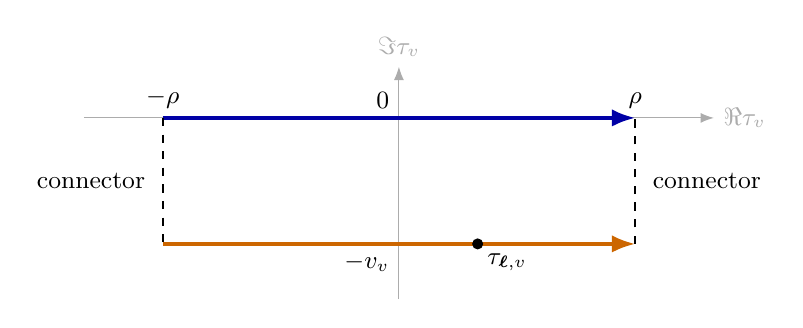
\begin{tikzpicture}[x=1cm,y=1cm,>=Latex,
 every node/.style={font=\small}]
 \draw[->,gray!65] (-4,0)--(4,0) node[right] {$\Re\tau_v$};
 \draw[->,gray!65] (0,-2.3)--(0,.65) node[above] {$\Im\tau_v$};
 \draw[very thick,blue!65!black,->] (-3,0)--(3,0);
 \draw[very thick,orange!80!black,->] (-3,-1.6)--(3,-1.6);
 \draw[dashed,thick] (-3,0)--(-3,-1.6);
 \draw[dashed,thick] (3,-1.6)--(3,0);
 \node[above] at(-3,0){$-\rho$};
 \node[above] at(3,0){$\rho$};
 \node[above left] at(0,0){$0$};
 \fill (1.0,-1.6) circle(2pt);
 \node[below right] at(1,-1.6){$\tau_{\boldsymbol\ell,v}$};
 \node[left] at(-3.1,-.8){connector};
 \node[right] at(3.1,-.8){connector};
 \node[below left] at(0,-1.6){$-v_v$};
\end{tikzpicture}

\caption{One coordinate of the finite angular deformation.
The real box has endpoints \(\pm\rho\), with \(\rho=1/8\);
its translated horizontal side passes through the critical point.
The two vertical sides are retained as connectors, with their
boundary orientations when comparing the horizontal integrals.
Here \(v_v=-\Im\tau_{\boldsymbol\ell,v}>0\).
Other coordinates can have intermediate downward displacements,
so their negative Fourier terms are kept in
\eqref{cta:connector}. The earlier infinite-charge estimate
uses real or translated-grid spectators, before this deformation.}
\label{cta:contour-figure}
\end{figure}

\subsection{Matching the geometric branch}
The analytic action is exactly the action of
\cite[Theorem~1.1]{Geometry}, not just a function with its
complete Hessian. Its derivative \eqref{cta:psi-definition}
agrees on every edge with that theorem, and the constants agree:
\(2G_0=v_{\rm oct}/\pi\), where \(v_{\rm oct}\) is the regular
ideal octahedron volume. This last equality also follows directly
from the Lobachevsky integral at \(\pi/4\).

Write \(n_v=\epsilon_v-2p_v\), with the retained parity
\(\epsilon_v\in\{-1,0,1\}\) in each actual disk frame.
The geometric theorem fills the original primitive slope
\(\mu_v+p_v\lambda_v\), with periods
\[
 U_v=-2\pi\Psi_{\tau_v}-\ii\epsilon_v\tau_v,\qquad
 V_v=2\ii\tau_v.
\]
Its unit-charge equation is
\(\Psi_{\tau_v}+\ii n_v\tau_v/(2\pi)=\ii\), precisely
\eqref{cta:fixedpoint} for \(\boldsymbol\ell=\mathbf1\).
The summed condition implies
\(\sqrt{d_v^2+n_v^2}\ge2^{25/2}>630\).
Furthermore \eqref{cta:tau-formula} gives
\[
 |\tau_{*,v}|\le
 \frac{2\pi}{(1-\delta)\sqrt{d_v^2+n_v^2}}<10^{-2}.
\]
Thus our critical point lies in the geometric theorem's
uniqueness chart. Its original filled metric is smooth,
complete and finite-volume, including zero powers at high-degree
vertices; every main cusp stays complete. Its absolute
fundamental-chain calculation gives
\(\Vol(S^3\setminus K_{\mathbf n})=2\pi\Rea\calC(\mathbf1)\).
There is no appeal here to a long-twist theorem for a zero
power, or to a formal exponentiated slope without metric completion.
Taking logarithms of the already nonzero
\eqref{cta:leading} proves Theorem~\ref{cta:main}.

\subsection{The centered main-meridian insertion}
The finite scalar ledger of \cite[Proposition~8.1]{Meridian}
separates exactly \(A_N(s)\) from the index-dependent factors
\(H_N/W_k\), the shifted crossing grids and the single closing
factor \(H_N(s)\). In the first-charge coefficient every grid
parameter has disappeared because \(c_{1,N}(\sigma)=1\).
The chirp has no remaining \(\sigma\)-dependence once its
recorded scalar is extracted.

It remains to integrate the second line of
\eqref{cta:packet-expansion} on the same joint contour.
For any fixed holomorphic insertion \(h(\boldsymbol\tau)\),
the normalized angular Gaussian evaluates it as
\(h(\boldsymbol\tau_*)+O(N^{-1})\): its linear Gaussian
term vanishes, and the quadratic term and its interaction
with the cubic phase contribute \(O(N^{-1})\).
The expansion to the next order and the fixed losses above
make this statement uniform on \(|s|\le R\).
Apply it to
\(-\pi s^2\sum_e\cot(\pi x_e(\boldsymbol\tau))\),
which already has the factor \(N^{-1}\).
The common first saddle correction cancels upon division
by \(F_N(1)\). The result is \eqref{cta:profile-formula}
with a uniform \(O_R(N^{-2})\) remainder.
In particular the wire values are those at the filled
critical point, not the complete values \(1/4\).

Both \(A_N\) and \(H_N\) are nonzero and bounded away from
zero on the fixed disk for large \(N\).
The ratio in \eqref{cta:profile-formula} tends uniformly
to one. This proves uniform eventual nonvanishing and
the remaining assertions of Theorem~\ref{cta:profile}.
No division by an unproved nonzero finite invariant was
used to establish the leading term.


\section{The directed degree-and-twist condition}\label{dt:criterion}
The root in this section is an order for evaluating the closed finite
contraction. It need not be the terminal root used to draw the original
knot. A nonroot vertex sends one polynomial to its parent; the last
vertex sends none. The following constants and inequalities reflect
that difference.

Put

\begin{equation}\label{dt:eq-1}
\begin{gathered}
a_0=\frac1{2\pi},\qquad k_0=2^{-16},\qquad
 R_0=\frac18,\qquad b_0=2^{-11},\qquad\\
 r_0=\frac1{16},\qquad t_0=2^{-14},\qquad
 \chi=1-\cos r_0.
\end{gathered}
\end{equation}

The parent-variable rectangle is

\begin{equation}\label{dt:eq-2}
\mathcal R=\{u:|\Re u|\le R_0,\ |\Im u|\le b_0\}.
\end{equation}

Choose any vertex as root and direct all edges toward it. For every
nonroot vertex choose a number

\begin{equation}\label{dt:eq-3}
0<c_v<k_0,
 \qquad
 \delta_v=\min\left\{\frac{b_0}2,
               \frac{c_v\chi}{4(1+c_v)}\right\}.
\end{equation}

These are parameters of the criterion. They can differ at every edge.
They are not asymptotic quantities to be inferred from the invariant.

Write \(q_v=1\) at a nonroot vertex and \(q_v=0\) at the root. If \(\mathrm{Ch}(v)\) is the
set of children, define

\begin{equation}\label{dt:eq-4}
\begin{aligned}
 a_v&=\frac{d_v}{2\pi},& b_v&=\frac{n_v}{2\pi},&
 D_v&=a_v-i b_v,\\
 A_v&=\frac2{\pi^2}
       \left(q_vk_0+\frac12\sum_{w\in\mathrm{Ch}(v)}c_w\right),&
 B_v&=16q_v+|\mathrm{Ch}(v)|,&
 C_v&=B_v+\frac{b_v^2}{4A_v}.
\end{aligned}
\end{equation}

There is at least one incidence at every vertex, so \(A_v,B_v\) are positive.
Let

\begin{equation}\label{dt:eq-5}
\delta_v^{\mathrm{in}}
      =\min\bigl(\{b_0\}\cup
                     \{\delta_w:w\in\mathrm{Ch}(v)\}\bigr)
\end{equation}

and set

\begin{equation}\label{dt:eq-6}
y_v=\min\left\{
 \frac{\delta_v^{\mathrm{in}}}2,
 \frac{t_0|D_v|}{4C_v},
 \frac{A_v\pi^2}{8(\pi|b_v|+t_0|D_v|)},
 \sqrt{\frac{A_v\pi^2}{8B_v}}
 \right\}.
\end{equation}

Finally define two action quantities

\begin{equation}\label{dt:eq-7}
\beta_v=\frac{210}{361}\frac{a_v}{|D_v|^2},
 \qquad
 \eta_v=\min\left\{
 \frac12t_0|D_v|y_v,
 \frac12A_v\pi^2,
 A_vr_0^2,
 \frac18a_vr_0^2
 \right\}.
\end{equation}

The criterion consists of the strict inequalities

\begin{equation}\label{dt:eq-8}
\boxed{\quad t_0|D_v|\ge2,\qquad
                 \beta_v<\frac{\eta_v}{2}\quad
                      \text{at every vertex},\quad}
\end{equation}

and, only at nonroot vertices,

\begin{equation}\label{dt:eq-9}
\boxed{\qquad
       \beta_v<(k_0-c_v)\chi.\qquad}
\end{equation}

It is a finite elementary test in the degrees, signed powers, root and
positive numbers \(c_v\). It uses no value of an unknown quantum invariant
and no assumed dominance of a global saddle. Its quantities are local:
\(A_v\) and the available strip depend on the child budgets, while the exact
child scalar will be divided out rather than estimated.


We say that the chosen root and numbers \(c_v\) satisfy the directed
criterion when \eqref{dt:eq-3}, \eqref{dt:eq-8} and \eqref{dt:eq-9} hold.
No numerical estimate of an invariant enters this definition.
The number \(\beta_v\) bounds the action lost in evaluating just the
current trace after exact child constants are divided out. The four
entries of \(\eta_v\) pay, respectively, for the infinite charge tail,
the original endpoints, localization to a real interval, and its
vertical connecting paths. The extra comparison \eqref{dt:eq-9} is used
only to produce an outgoing real bound.

\subsection{The full kernel with a fixed parent angle}\label{dt:sec-2}

The basis \(e_k\), trace \(\phi_\sigma\), paired factor \(W_k\) and
edge phase \(\psi\) are those of Sections~\ref{cta:finite}--\ref{cta:angular}.
The turn retains the scalar \(\gamma_e\) fixed by the original edge
orientation; it stays in the exact scalar factors of the contraction.
Lemma~\ref{cta:norms} and the complex edge calculation in
Section~\ref{cta:edge} apply before either degree-and-twist condition.
Use the exact full kernel

\begin{equation}\label{dt:eq-13}
K_N(t,u;s)=\sum_{k=0}^{N-1}
       e_k(-2\cos t)e_k(-2\cos u)\frac{H_N(s)}{W_k(s)}.
\end{equation}

The definitions of \(e_k,W_k\) and the fixed anti-diagonal trace metric are
unchanged. It is a polynomial of degree at most \(N-1\) in each of
\(-2\cos t\) and \(-2\cos u\), hence has trigonometric degree at most
\(N-1\) in either angle.
The paired factors and their inverses are bounded for fixed \(|s|\le R<1\).
Every inequality below permits a polynomial factor in N.

The full-kernel real estimate is

\begin{equation}\label{dt:eq-14}
|K_N(t,u;s)|\le C_RN^{A_R}
   e^{N\{2G_0-k_0[(1-\cos t)+(1-\cos u)]\}},
                 \qquad t,u\in[-\pi,\pi].
\end{equation}

To verify this, split the sum at \(I=[1/5,3/10]\).
On \(I\), \eqref{cta:raw} gives angular loss
\(\sin^2(t/2)/160\) at each end. The positive zero-angle sum
has rate \(2G_0\). Outside \(I\), the full polynomial bound
has loss \(\eta_K=\pi/200\), including high-index derivatives.
Since \(4k_0<\eta_K\) and \(2k_0<1/160\), both parts obey
\eqref{dt:eq-14}. The bounded paired insertion changes only its
polynomial prefactor.

The conditional estimate needed here is

\begin{equation}\label{dt:eq-15}
|K_N(t+iy,u;s)|\le C_RN^{A_R}
 e^{N\{\Re\psi(0,u)-k_0(1-\cos t)+16y^2\}},
 \quad u\in\mathcal R,\quad t\in[-\pi,\pi],\quad |y|\le b_0.
\end{equation}

The parent parameter ranges over the rectangle \(\mathcal R\).
The constant term is the conditional phase \(\psi(0,u)\); retaining it
is necessary when the exact child constants are divided out.

Here is a proof from the original finite kernel. Split the indices into
\(I=[1/5,3/10]\) and its complement. The complementary full polynomial, by Lemma~\ref{cta:norms} and \eqref{cta:discard}, has the single-edge loss \(\eta_K=\pi/200\), including high
indices and their complete derivatives. Its ellipse bound is

\begin{equation}\label{dt:eq-16}
C_RN^{A_R}
       e^{N\{2G_0-\eta_K+|y|+|\Im u|\}}.
\end{equation}

The edge Hessian in \eqref{cta:edge-Hessian} gives, on the radius 1/4 bidisk,

\begin{equation}\label{dt:eq-17}
|\psi_{tt}+a_0|\le a_0/50,
 \quad |\psi_{uu}+a_0|\le a_0/50,
 \quad |\psi_{tu}|\le a_0/50,
 \quad \psi_t(0,u)=\psi_u(t,0)=0.
\end{equation}

In particular \(|\psi(0,u)-2G_0|\le |u|^2/10\). Hence \eqref{dt:eq-16} is smaller
than \eqref{dt:eq-15}: the sum \(b_0+b_0+(R_0^2+b_0^2)/10+2k_0\) is less
than \(\eta_K/2\). All these constants are independent of the tree.

For the retained indices write \(u=a+ib\). Their factors at \(a\) are positive.
If \(r_j=\cos(2\pi(j+1/2)/N)\), then \(r_j>-1/3\) and
\(r_j+\cos a>253/384\). Along \(|a|\le1/8,\ |b|\le2^{-11}\), the denominator
\(r_j+\cos(a+ib)\) has modulus greater than \(3/5\), and

\begin{equation}\label{dt:eq-18}
\left|\frac{d^2}{du^2}\log(r_j+\cos u)\right|
 =\left|\frac{-r_j\cos u-1}{(r_j+\cos u)^2}\right|<9.
\end{equation}

The first derivative at real a is real. Integrating vertically therefore
gives the actual finite-product estimate

\begin{equation}\label{dt:eq-19}
|e_k(-2\cos(a+ib))|
       \le e_k(-2\cos a)e^{5Nb^2},\qquad k/N\in I.
\end{equation}

At the other end retain the original product bound

\begin{equation}\label{dt:eq-20}
|e_k(-2\cos(t+iy))|
   \le e^2e_k(-2)e^{N[-\alpha\sin^2(t/2)+11y^2]},
                       \qquad \alpha=1/160>1/250.
\end{equation}

The positive retained sum at \((0,a)\) is bounded by a polynomial times
\(\exp(N\psi(0,a))\), uniformly for real \(|a|\le1/8\). This is the positive one-edge Laplace estimate in Section~\ref{cta:edge}: its unique critical wire is

\begin{equation}\label{dt:eq-21}
\tan^2(\pi x)=\frac1{1+\tan^2(a/2)},
\end{equation}

which stays in the interior of \(I\). Its second derivative stays negative
on this fixed real compact. Equations \eqref{dt:eq-19}--\eqref{dt:eq-20}, and the second bound
in \eqref{dt:eq-17}, consequently give

\begin{equation}\label{dt:eq-22}
|K_{N,I}(t+iy,u;s)|\le C_RN^{A_R}
 e^{N\{\Re\psi(0,u)-\alpha\sin^2(t/2)+11y^2+6b^2\}}.
\end{equation}

For \(|t|\ge1/8\),

\begin{equation}\label{dt:eq-23}
6b_0^2<\frac{\alpha}{2}\sin^2(1/16),\qquad
                         2k_0<\alpha/2.
\end{equation}

For example \(\sin(1/16)>1/(8\pi)\), \(\pi^2<10\) and \(\alpha>1/250\) already
prove the first inequality. This proves \eqref{dt:eq-15} in this range.

For \(|t|\le1/8\), \eqref{cta:edge-expansion} gives the exact
nonzero edge asymptotic on the 1/4 bidisk. Both \(u\) and \(t+iy\) lie strictly
inside that disk. Integrating the first bound of \eqref{dt:eq-17} gives \eqref{dt:eq-15} there.
The original lattice currents and \eqref{dt:eq-16} are exponentially smaller.
In particular the full kernel, uniformly on this smaller rectangle
product, retains

\begin{equation}\label{dt:eq-24}
K_N(t,u;s)=N^{-3/2}a_e(t,u)e^{N\psi(t,u)}
                         (1+O_R(N^{-1})),
\end{equation}

with the original nonzero holomorphic leading amplitude and midpoint
normalization. The outside physical edge gamma is not included in \(a_e\).

\subsection{The exact recursion may be rooted anywhere}\label{dt:sec-3}

Lower the fixed Frobenius pairing at every vertex of the original closed
source. Every physical turn then identifies equal Newton indices and
retains its factor \(\gamma_e H_N/W_k\). The resulting finite scalar is a
sum over the original edge indices of a product of the original vertex
trace tensors. Choosing a root merely specifies the order of these
finite contractions. It does not move a cut through a tangle, commute
open operators or change a framing.

Consequently the exact recursions of \cite[Theorem~7.1]{Meridian} hold for any chosen root:

\begin{equation}\label{dt:eq-25}
M_{v,N}(u)=\gamma_{e_v}(s)\,
 \mathcal D_{n_v,\sigma_v,N}^{(t)}
 \left[K_N(t,u;s)\prod_{w\in\mathrm{Ch}(v)}M_{w,N}(t)\right]
\end{equation}

at a nonroot vertex, where
\(\mathcal D_{n,\sigma,N}[f]=\phi_\sigma(R_\sigma^n f)\)
uses the actual physical crossing polynomial and its Cartan scalar.
At the root the recursion is

\begin{equation}\label{dt:eq-26}
Z_N=\mathcal D_{n_o,\sigma_o,N}^{(t)}
                  \left[\prod_{w\in\mathrm{Ch}(o)}M_{w,N}(t)\right]
\end{equation}

at the root. The original global closing, framing and reference factors of \cite[Proposition~8.1]{Meridian},
and the original single reduced cut \(H_N\), remain outside \eqref{dt:eq-26}. Edge
gammas are counted once. The exact normal value \(\sigma_v=0\) and the moving
values \(\pm s\) retain their actual orientation types.

Each message is an even trigonometric polynomial of degree at most \(N-1\)
in \(u\), regardless of the subtree. There is no discarded-source error in
\eqref{dt:eq-25}--\eqref{dt:eq-26}.

\begin{figure}[t]
\centering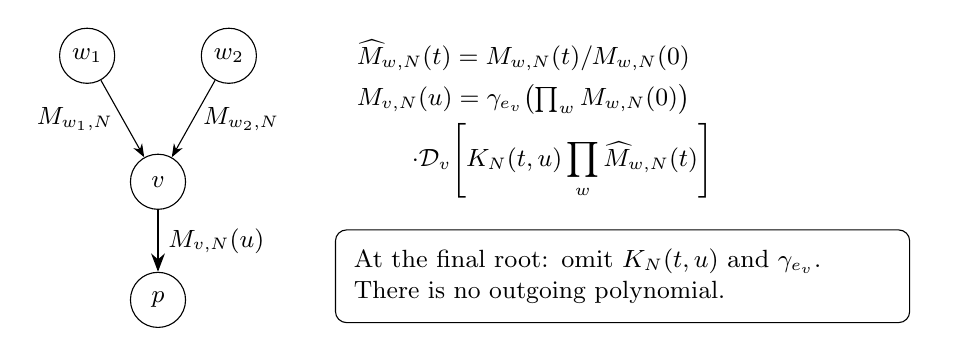
\begin{tikzpicture}[x=1cm,y=1cm,>=Stealth,vertex/.style={circle,draw,fill=white,minimum size=7mm,inner sep=1pt},every node/.style={font=\small}]
\node[vertex] (a) at (-4,1.6) {$w_1$};
\node[vertex] (b) at (-2.2,1.6) {$w_2$};
\node[vertex] (v) at (-3.1,0) {$v$};
\node[vertex] (p) at (-3.1,-1.5) {$p$};
\draw[->] (a)--node[left] {$M_{w_1,N}$} (v);
\draw[->] (b)--node[right] {$M_{w_2,N}$} (v);
\draw[->,thick] (v)--node[right] {$M_{v,N}(u)$} (p);
\node[anchor=west,align=left,text width=7.4cm] at (-.7,.8)
 {$\widehat M_{w,N}(t)=M_{w,N}(t)/M_{w,N}(0)$\\[4pt]
 $M_{v,N}(u)=\gamma_{e_v}\!\left(\prod_wM_{w,N}(0)\right)$\\[2pt]
 $\displaystyle\hspace{7mm}\cdot\mathcal D_v\!\left[K_N(t,u)\prod_w\widehat M_{w,N}(t)\right]$};
\node[draw,rounded corners,align=left,text width=6.8cm,inner sep=7pt] at (2.8,-1.2)
 {At the final root: omit $K_N(t,u)$ and $\gamma_{e_v}$. There is no outgoing polynomial.};
\end{tikzpicture}

\caption{Edges point toward the vertex whose trace is evaluated next.
The exact numbers \(M_{w,N}(0)\) are factored out before applying that
trace. The outgoing polynomial is then divided by its own exact value
at zero. Only a nonroot vertex must supply an outgoing real-decay bound;
the final root evaluates a scalar. This diagram describes contraction
order, not an isotopy of the knot.}\label{dt:recursion-figure}
\end{figure}

\subsection{The phase class and the variable envelopes}\label{dt:sec-4}

The inductive analytic class is

\begin{equation}\label{dt:eq-27}
h_v(0)=h'_v(0)=0,\qquad h_v(-u)=h_v(u),\qquad
 |h_v''(u)+a_0|\le a_0/20,\quad u\in\mathcal R.
\end{equation}

The leading normalized amplitude \(\alpha_v(u)/\alpha_v(0)\) is holomorphic
and nonzero on a neighborhood of the required smaller compact. Exact
subtree constants are retained:

\begin{equation}\label{dt:eq-28}
\frac{M_{v,N}(u)}{M_{v,N}(0)}
 =\frac{\alpha_v(u)}{\alpha_v(0)}e^{Nh_v(u)}(1+O(N^{-1})),
                     \quad u\in\mathcal R.
\end{equation}

As usual a slightly smaller rectangle can be used for fixed derivative
estimates; the strict margins permit an initially slightly larger one.

The global assertions attached to \(c_v\) are

\begin{equation}\label{dt:eq-29}
\left|\frac{M_{v,N}(t)}{M_{v,N}(0)}\right|
          \le CN^A e^{-Nc_v(1-\cos t)},
                         \quad t\in[-\pi,\pi],
\end{equation}

\begin{equation}\label{dt:eq-30}
\left|\frac{M_{v,N}(t+iy)}{M_{v,N}(0)}\right|
 \le CN^A e^{N[-(c_v/2)(1-\cos t)+y^2]},
                      \quad |y|\le\delta_v.
\end{equation}

For canonical representatives of degree less than \(N\), the real sup,
Chebyshev and full value-and-first-derivative norms differ by polynomial
factors, by Lemma~\ref{cta:norms}. A product of degree a fixed multiple
of \(N\) is first bounded in its real sup norm and then folded in the
correct quotient; no equivalence with finite node data is asserted for
an unreduced higher-degree polynomial. In particular the reduction and
trace retain the repeated-root normals.

Here is the passage from the real bound to the strip. Write the
normalized message as a Laurent polynomial \(P(e^{\ii t})\), of powers
between \(-m\) and \(m\), where \(m<N\). The subharmonic function
\(\log|z^mP(z)|\) on the unit disk is bounded by the harmonic
function \(\log(CN^A)-Nc_v+Nc_v\Re z\). Substitute
\(z=e^{-y+\ii t}\) and divide by \(|z|^m\); for negative \(y\)
use the reciprocal polynomial. Since \(1-e^{-|y|}\le|y|\), this gives

\begin{equation}\label{dt:eq-31}
|M_{v,N}(t+iy)/M_{v,N}(0)|
 \le CN^A e^{N[-c_v(1-\cos t)+(1+c_v)|y|]}.
\end{equation}

For \(|t|\ge r_0\) use \eqref{dt:eq-3}. For \(|t|<r_0\) use the rectangle expansion and

\begin{equation}\label{dt:eq-32}
\Re h_v(t+iy)\le
       -\frac{19a_0}{40}t^2+\frac{21a_0}{40}y^2.
\end{equation}

Both arguments give \eqref{dt:eq-30}, without a conjectured quadratic estimate for
an individual high Newton basis element.

Assume the children satisfy \eqref{dt:eq-27}--\eqref{dt:eq-30}. At a nonroot vertex set

\begin{equation}\label{dt:eq-33}
A_v^{\mathrm{loc}}(t,u)=\psi(t,u)+\sum_wh_w(t),
 \quad
 C_{v,\ell}(u)=\operatorname{stat}_t
       \{A_v^{\mathrm{loc}}(t,u)+ib_vt^2/2-i\ell t\}.
\end{equation}

At the root omit \(\psi\) and \(u\). There are \(d_v\) incidences in \(t\). Hence

\begin{equation}\label{dt:eq-34}
A_v^{\mathrm{loc}}(t,u)=\psi(0,u)-a_vt^2/2+E_v(t,u),
       \quad |E_{v,tt}|,\ |E_{v,t}/t|\le a_v/20.
\end{equation}

The root constant in this formula is zero. For \(0\le\ell\le L_v=\lfloor t_0|D_v|\rfloor\)
the equation \(D_vt=-i\ell+E_{v,t}\) contracts in \(|t|\le b_0\). Indeed
\(t_0+b_0/20<b_0\). The actual solutions lie in the smaller disk
\(|t|\le t_0/(19/20)\), leaving room for the translated contours.

Writing \(E_{v,t}=tQ_v\), with \(|Q_v|\le a_v/20\), gives
\(t_{v,\ell}=-\ii\ell/(D_v-Q_v)\). Its imaginary part is
\(-\ell\Re(D_v-Q_v)/|D_v-Q_v|^2\). The numerator lies
between \(19a_v/20\) and \(21a_v/20\), and the denominator
between \((19|D_v|/20)^2\) and \((21|D_v|/20)^2\).
Therefore

\begin{equation}\label{dt:eq-35}
\frac{380}{441}\frac{\ell a_v}{|D_v|^2}
 \le-\Im t_{v,\ell}\le
 \frac{420}{361}\frac{\ell a_v}{|D_v|^2},
\end{equation}

also for complex parent \(u\). No child phase is asserted to be real on
the real axis. Its nonlinear derivative is \(t\) times a function bounded
by \(a_v/20\), so the real part of the denominator remains positive.

The normalized phase \(h_v=C_{v,1}(u)-C_{v,1}(0)\) satisfies

\begin{equation}\label{dt:eq-36}
h'_v=\psi_u(t_{v,1},u),\qquad
 h''_v=\psi_{uu}
       -\frac{\psi_{ut}^2}{A_{v,tt}^{\mathrm{loc}}+ib_v}.
\end{equation}

Using \eqref{dt:eq-17} and \(|A_{v,tt}^{\mathrm{loc}}+ib_v|\ge(19/20)|D_v|\ge(19/20)a_0\) proves \eqref{dt:eq-27},
since \(1/50+20/(19\cdot2500)<1/20\). This is uniform on the rectangle.
Charge ordering and the current-vertex drop are

\begin{equation}\label{dt:eq-37}
\Re C_{v,\ell}(u)\le\Re C_{v,1}(u)
  -\frac{190}{441}\frac{a_v}{|D_v|^2}(\ell^2-1),
 \quad
 0\le\Re\psi(0,u)-\Re C_{v,1}(u)\le\beta_v.
\end{equation}

At the root again replace \(\psi(0,u)\) by zero.

\subsection{Actual trace tails with the directed budgets}\label{dt:sec-5}

Divide every child by its exact nonzero value \(M_{w,N}(0)\). The induction
uses those complex constants exactly; it never estimates them by their
complete-source magnitudes. Equations \eqref{dt:eq-15} and \eqref{dt:eq-30} imply

\begin{equation}\label{dt:eq-38}
|\text{normalized trace input}(t+iy,u)|
 \le CN^A
   e^{N[\Re\psi(0,u)-A_vt^2+B_vy^2]},
                      \quad |y|\le\delta_v^{\mathrm{in}}.
\end{equation}

The root constant is zero. The factor \(2/\pi^2\) in \eqref{dt:eq-4} is exactly the
inequality \(1-\cos t\ge2t^2/\pi^2\) on the original interval.

Apply the exact trace formula \eqref{cta:trace} and the residue
calculation of Section~\ref{ct:trace-section} to this normalized input.
Here the rectangle has height \(y_v\). The input is an even
trigonometric polynomial of degree a fixed multiple of \(N\), so
that calculation applies without reduction to a distinct-node model.
The paired charge coefficient is \eqref{dt:eq-39}, with first
coefficient exactly one. All endpoint currents, including the
zero-mode currents, remain to be estimated below.

For \(\ell>L_v\), moving the single-grid rectangle by \(y_v\) costs, after
maximizing the chirp term in the real variable, at most \(C_v y_v^2\).
Since \(\ell>L_v\) implies \(\ell>t_0|D_v|\), \eqref{dt:eq-6} gives a tail loss at least

\begin{equation}\label{dt:eq-40}
t_0|D_v|y_v-C_vy_v^2\ge\frac12t_0|D_v|y_v.
\end{equation}

Successive charges have the additional factor \(\exp(-Ny_v)\). The exact
fixed-compact growth of \eqref{dt:eq-39} is absorbed for all sufficiently large N.
This starting level may depend on the fixed vertex.

At an original endpoint \(\pm\pi\), the chirp and finite-charge connectors cost
at most

\begin{equation}\label{dt:eq-41}
(\pi|b_v|+t_0|D_v|)y_v+B_vy_v^2
                            \le A_v\pi^2/4.
\end{equation}

Thus their loss is at least \(A_v\pi^2/2\). This includes the original
zero-mode current. Nothing is inferred by dropping the endpoint terms
of the nonperiodic chirp.

For a retained charge, restrict its real integral to \([-r_0,r_0]\).
Its complement loses \(A_vr_0^2\) by \eqref{dt:eq-38}. Translate the retained interval
to \(\Im t_{v,\ell}\). Its endpoints remain in the analytic rectangle. The
original local Young inequality, now on this larger real interval,
is

\begin{equation}\label{dt:eq-42}
\begin{aligned}
 \Re\{A_v^{\mathrm{loc}}(t-iz,u)+ib_v(t-iz)^2/2-i\ell(t-iz)\}
 &\le\Re\psi(0,u)-a_vt^2/8\\
 &\quad+\left[\frac{21}{40}a_v+
                 \frac{2b_v^2}{(14/5)a_v}\right]z^2-\ell z.
\end{aligned}
\end{equation}

For \(0\le z\le-\Im t_{v,\ell}\), the last line after its quadratic term is
at most \(-\ell z/8\), since \((420/361)\max(21/40,5/7)=300/361<7/8\).
Every such connector therefore loses at least \(a_vr_0^2/8\).
The translated horizontal saddle has negative real quadratic part
at most \(-(19/20)a_v\). The physical sine factor is nonzero at \(t_{v,\ell}\).

Equations \eqref{dt:eq-40}--\eqref{dt:eq-42} give an error of at most
\(CN^A\exp N[\Re\psi(0,u)-\eta_v]\). Nonminimal charges are their saddle
terms plus this absolute error; no relative approximation is asserted
at a much lower nonminimal action. Conditions \eqref{dt:eq-8} and \eqref{dt:eq-37} put the
whole conditional error strictly below the first charge. Equation
\eqref{dt:eq-39} gives its nonzero coefficient for both parities. This establishes
\eqref{dt:eq-28} and nonvanishing of the exact \(M_{v,N}(0)\).

For the child inputs, their exact analytic logarithms differ from the
limiting phases by \(O(N^{-1})\), with fixed derivatives on the required
smaller compact. The finite product of those corrections is retained
in the amplitude, or moves the saddle by \(O(N^{-1})\). As the tree is fixed,
it spends no new exponential budget. The leading amplitude is a product
of nonzero edge, child and Gaussian factors. All N-dependent physical
crossing and carrier phases remain in \(M_{v,N}(0)\); its normalized leading
amplitude does not conceal such phases.

The full physical trace and the first-charge approximation are
holomorphic in the formal meridian variables. As in the original
proof, first take parameter circles avoiding collisions and then apply
the maximum principle to their whole difference. This covers every
actual \(\sigma_v=0,\pm s\), including normal limits. No isolated divided
current is declared removable without its companions.

\subsection{Regenerating the outgoing real bound}\label{dt:sec-6}

Lemma~\ref{cta:norms} compares the real sup norm, the
Chebyshev norm, and the complete value-and-first-derivative norm by
polynomial factors. It also bounds the physical fixed-power crossing
and the full quotient trace. These estimates apply to polynomial
products of degree a fixed multiple of \(N\); that multiple can depend
on the degree of this fixed vertex. For real \(u\), \eqref{dt:eq-14},
the polynomial real sup bounds of the normalized children, the actual
fixed-power crossing polynomial, Chebyshev folding in the correct
quotient, and the full top-coefficient functional give

\begin{equation}\label{dt:eq-43}
|M_{v,N}(u)|\le CN^A
       \left|\prod_wM_{w,N}(0)\right|
                  e^{N[2G_0-k_0(1-\cos u)]}.
\end{equation}

This retains repeated-root derivatives and all fixed normals. Dividing
by the nonzero first-charge value at zero costs at most \(\beta_v\). For
\(|u|\ge r_0\), \eqref{dt:eq-9} absorbs that cost and yields \eqref{dt:eq-29}. For \(|u|<r_0\), \eqref{dt:eq-28}
and \eqref{dt:eq-32} give the stronger estimate, since \(c_v<k_0\ll19a_0/20\).
Equation \eqref{dt:eq-30} follows by Section~\ref{dt:sec-4}. Thus the induction closes with
the selected directed budgets, rather than a common decay constant.

There is no outgoing real bound at the final root. Imposing \eqref{dt:eq-9} there
would be an unnecessary restriction. Its only normalization comparison
is the conditional trace estimate \eqref{dt:eq-8}.

\subsection{Original action, geometry, and scope}\label{dt:sec-7}

Restore the exact subtree constants successively. Stationary
elimination in \eqref{dt:eq-33} gives the original joint equations

\begin{equation}\label{dt:eq-44}
\sum_{e\sim v}\psi_{e,\tau_v}
                      +\frac{in_v\tau_v}{2\pi}=i.
\end{equation}

The exact child constants telescope to the original critical value

\begin{equation}\label{dt:eq-45}
\calC(\mathbf1)=\operatorname{stat}_{\boldsymbol\tau}
 \left[\sum_e\psi_e+
       \frac{i}{4\pi}\sum_vn_v\tau_v^2-i\sum_v\tau_v\right].
\end{equation}

Back-substitute from the final root: its first-charge angle belongs to
the rectangle, so each child's selected parent value does also, and
the same statement continues down the finite tree. Every restored angle
has modulus at most \(1/[(19/20)|D_v|]\). Thus the vector satisfying
\eqref{dt:eq-44} lies inside the full simultaneous small-angular uniqueness
polydisk, not just the conditional disks used during elimination.
The existing contraction identifies it with the same branch as the
marked positive charge path of \cite[Theorem~1.1]{Geometry}. In fact
\(20/(19|D_v|)<10^{-2}\). Indeed
\eqref{dt:eq-8} implies

\begin{equation}\label{dt:eq-46}
\sqrt{d_v^2+n_v^2}=2\pi|D_v|\ge 2\pi\,2^{15}>630.
\end{equation}

\cite[Theorem~1.1]{Geometry} applies with no sum condition.
The edge functions agree: their derivatives are \eqref{cta:psi-definition} and
their complete values satisfy \(2G_0=v_{\rm oct}/\pi\), as in
Section~\ref{cta:conclusion}. Write \(n_v=\epsilon_v-2p_v\), with
\(\epsilon_v\in\{-1,0,1\}\), in the original disk frame. The
primitive periods supplied by the geometric theorem are
\[
 U_v=-2\pi\Psi_{\tau_v}-\ii\epsilon_v\tau_v,
 \qquad V_v=2\ii\tau_v.
\]
Equation \eqref{dt:eq-44} therefore gives the full continued relation
\(U_v+p_vV_v=-2\pi\ii\). The imported theorem proves its primitive
winding, smooth metric completion, and complete main cusp; we do not
infer these facts from an exponentiated equation.
Its original ordered two-octahedron cut, odd seam and calibrated action identify \(2\pi\Re\calC(\mathbf1)\) with the volume of the actual
filled knot complement. This is a geometric input, not a deduction
from the quantum saddle alone.

There are \(|E|\) edge Gaussians \(N^{-3/2}\) and \(|V|\) trace Gaussians \(N^{3/2}\);
\(|V|=|E|+1\) leaves the original \(N^{3/2}\) power with nonzero amplitude.
The exact first Fourier coefficient is one. The retained edge insertion
has leading value one, and the scalar ledger remains precisely \eqref{dt:scalars}.
At \(s=0\), all edge gammas and paired insertions equal one.
The exact outside scalar is
\[
 \Omega_N=\theta_d^{-w(D)}\prod_vC_{N,n_v}(0)
       =q_N^{d^2(2w(D)+\sum_v n_v)/4},
 \qquad \theta_d=q_N^{-d^2/2}.
\]
The remaining leading coefficient is independent of \(N\), nonzero,
and the same through both parities. This proves the full leading
asymptotic in Theorem~\ref{dt:main}.
For bounded \(s\), the first-charge coefficient is still one, the
paired insertion has leading value one, and all normalized leading
amplitudes are unchanged. Restoring the exact scalar ledger of
\cite[Proposition~8.1]{Meridian} gives \(A_N(s)H_N(s)\).
The finite product of relative \(1+O_R(N^{-1})\) factors proves
\eqref{dt:profile}. Its nonvanishing follows uniformly on every
fixed disk \(R<1\), since \(A_N\) and \(H_N\) have no zeros there.
Together with the geometric identification above this proves
Theorem~\ref{dt:main}.

The criterion allows different strip and real-decay budgets and a
different choice of final vertex. It is not the assertion that arbitrary
capped short-twist islands can be substituted as black-box messages.
Such an island requires a multi-boundary version of the conditional
normalization proved here for an actual edge. The one-edge estimates proved here do not supply that extension.

\section{Consequences and examples}\label{dt:sec-8}


\subsection{A star under the summed condition}
In a star with \(d\) terminal vertices, central power zero and terminal
powers \(n\), the sum in \eqref{cta:sum} is
\[
 \mathfrak S=\frac1d+\frac{d}{1+n^2}.
\]
Taking \(d\ge2^{27}\) and \(|n|\ge\sqrt{2^{27}d}\) gives
\(\mathfrak S\le2^{-26}\). The diagram must still satisfy the endpoint
condition of Section~\ref{cta:intro}; the numerical inequality alone
does not give that condition. This example uses only
Theorems~\ref{cta:main} and~\ref{cta:profile}.

\subsection{A uniform degree-or-twist alternative}

The directed criterion has the following simple consequence:

\begin{equation}\label{dt:eq-47}
|n_v|\ge2^{27}\quad\text{at every vertex}
             \quad\Longrightarrow\quad\text{Theorem~\ref{dt:main}}.
\end{equation}

This sufficient constant is independent of the number of vertices,
their degrees and the choice of root. Here is a proof covering all
degrees simultaneously. Choose \(c_v=k_0/2\) at every nonroot vertex
and write \(\delta\) for their common value in \eqref{dt:eq-3}. The elementary
cosine estimate gives

\begin{equation}\label{dt:eq-48}
\chi\ge\frac{r_0^2}{2}-\frac{r_0^4}{24}
       =2^{-9}\frac{3071}{3072}>2^{-10},\qquad
                          \delta>2^{-30}.
\end{equation}

At any vertex, including the root, put
\(\mathcal R_v=\sqrt{d_v^2+n_v^2}\). Then

\begin{equation}\label{dt:eq-49}
A_v\ge\frac{k_0d_v}{2\pi^2},\qquad B_v\le16d_v,
 \qquad C_v\le\frac{\mathcal R_v^2}{8k_0d_v}.
\end{equation}

For the last inequality use \(16\le1/(8k_0)\). Each of the four
branches of the minimum in \eqref{dt:eq-6} consequently has the following lower
bound, respectively:

\begin{equation}\label{dt:eq-50}
\frac\delta2,\qquad
 \frac{t_0k_0d_v}{\pi\mathcal R_v},\qquad
 \frac{k_0d_v}{16\mathcal R_v},\qquad 2^{-12}.
\end{equation}

The second displayed quantity is smaller than the third and fourth.
For the third bound, use
\(\pi|b_v|+t_0|D_v|\le\mathcal R_v(1+t_0/\pi)/2\).
Thus every branch of \eqref{dt:eq-7}, not just its tail branch, is bounded below by

\begin{equation}\label{dt:eq-51}
\eta_v\ge\min\left\{
       \frac{t_0\mathcal R_v\delta}{8\pi},
       \frac{t_0^2 k_0d_v}{4\pi^2}\right\}.
\end{equation}

Indeed the second entry here is smaller than each of the other three
entries in \eqref{dt:eq-7}, by their explicit values and \(t_0\ll r_0\).
On the other hand

\begin{equation}\label{dt:eq-52}
\beta_v=\frac{420\pi}{361}\frac{d_v}{\mathcal R_v^2}
                       <\frac{4d_v}{\mathcal R_v^2}.
\end{equation}

For comparison with half the first entry of \eqref{dt:eq-51}, it suffices that
\(\mathcal R_v^2>64\pi/(t_0\delta)\), since \(d_v\le\mathcal R_v\).
The right side is less than \(2^{52}\), using \(\pi<4\) and \eqref{dt:eq-48}.
For comparison with half the second entry it suffices that
\(\mathcal R_v^2>32\pi^2/(t_0^2k_0)\), whose right side is less
than \(2^{53}\), since \(\pi^2<10\). Both inequalities follow
strictly from \(\mathcal R_v^2\ge n_v^2\ge2^{54}\).
The charge-cut condition in \eqref{dt:eq-8} follows as well.

For the outgoing patch, the sharper elementary estimate is

\begin{equation}\label{dt:eq-53}
\beta_v\le\frac{210\pi}{361|n_v|}
 \le\frac{330}{361}\,2^{-26}
 <\frac{3071}{3072}\,2^{-26}
 \le\frac{k_0}2\chi.
\end{equation}

Here \(\pi<22/7\),
\(d_v/(d_v^2+n_v^2)\le1/(2|n_v|)\), and the displayed rational
comparison prove \eqref{dt:eq-9} for every degree. This completes the corollary
without a numerical scan or a threshold depending on the tree.

The same proof gives a mixed condition, chosen independently at each
vertex:

\begin{equation}\label{dt:eq-53a}
\boxed{\qquad
       d_v\ge2^{28}\quad\text{or}\quad |n_v|\ge2^{27}
               \qquad\text{for every }v.\qquad}
\end{equation}

Under the degree alternative, \(\mathcal R_v^2\ge d_v^2\ge2^{56}\)
proves the same two tail comparisons, while

\begin{equation}\label{dt:eq-53b}
\beta_v\le\frac{420\pi}{361d_v}
             \le\frac{330}{361}\,2^{-26}
                    <\frac{k_0}2\chi
\end{equation}

is the same outgoing patch bound. Neither alternative needs to hold
uniformly over all vertices. In particular, the high-degree vertices
may retain any fixed signed powers, including zero and small nonzero
powers. No sum over the number of such vertices occurs.

Here is a precise extension construction illustrating that freedom.
Start with any fixed ordered circle-tree core whose original endpoint
pairing closes to a knot and has no internal closed component. Retain
all its fixed signed powers. At every core vertex choose one of its
actual product slots next to its crossing box and insert a consecutive
stack of an even number \(B\ge2^{28}\) of new terminal pieces. Every
new leaf has a fixed odd power satisfying

\begin{equation}\label{dt:eq-53c}
|n_{\mathrm{leaf}}|\ge2^{27}+1.
\end{equation}

The physical quarter-turn of an odd two-strand braid has diagonal
pairing \(X=\{02,13\}\); this pairing is invariant under the
quarter-turn. An even ordered stack of these leaves has the through
pairing \(I=\{03,12\}\) and creates no internal circle. Inserting it
in the specified slot therefore preserves the original local endpoint
pairing in that actual frame. This is a pairing calculation, not an
isotopy removing the new tangles. At the original closing box the same
insertion takes place inside its local ball. An added terminal leaf may
then be chosen as the recursive root using the original closed-collar
move with its induced frame reversal and factor order retained.

Thus the resulting diagram is again a knot, while its knot type may
change. Each old vertex now satisfies the degree alternative and each
new leaf satisfies the twist alternative in \eqref{dt:eq-53a}. The resulting actual
knot complement is hyperbolic and satisfies Theorem~\ref{dt:main}. The number and
arrangement of prescribed short-power vertices are arbitrary but fixed;
the number \(B\) does not depend on their total count.

\begin{figure}[t]
\centering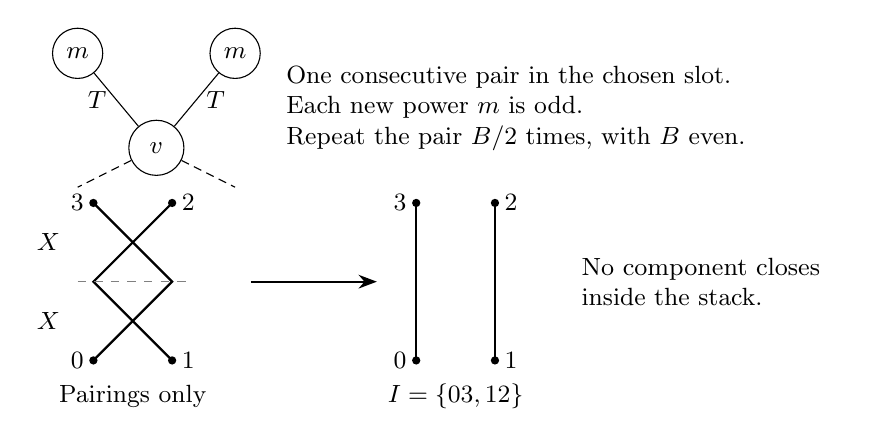
\begin{tikzpicture}[x=1cm,y=1cm,>=Stealth,every node/.style={font=\small}]
\node[circle,draw,minimum size=7mm] (v) at (-3,1.5) {$v$};
\node[circle,draw,minimum size=6mm] (l) at (-4,2.7) {$m$};
\node[circle,draw,minimum size=6mm] (r) at (-2,2.7) {$m$};
\draw (v)--node[left] {$T$}(l);
\draw (v)--node[right] {$T$}(r);
\draw[densely dashed] (v)--(-4,1);
\draw[densely dashed] (v)--(-2,1);
\node[align=left,text width=6.7cm] at (2,2)
 {One consecutive pair in the chosen slot.\\Each new power $m$ is odd.\\Repeat the pair $B/2$ times, with $B$ even.};
\begin{scope}[shift={(-3.8,-1.2)}]
\draw[thick] (0,0)--(1,1)--(0,2);
\draw[thick] (1,0)--(0,1)--(1,2);
\draw[dashed,gray] (-.2,1)--(1.2,1);
\foreach \x/\y in {0/0,1/0,0/2,1/2}{\fill (\x,\y) circle(1.5pt);}
\node[left] at (0,0) {$0$};\node[right] at (1,0) {$1$};
\node[right] at (1,2) {$2$};\node[left] at (0,2) {$3$};
\node[left] at (-.3,.5) {$X$};\node[left] at (-.3,1.5) {$X$};
\node at (.5,-.45) {Pairings only};
\end{scope}
\draw[->,thick] (-1.8,-.2)--(-.2,-.2);
\begin{scope}[shift={(.3,-1.2)}]
\draw[thick] (0,0)--(0,2);\draw[thick] (1,0)--(1,2);
\foreach \x/\y in {0/0,1/0,0/2,1/2}{\fill (\x,\y) circle(1.5pt);}
\node[left] at (0,0) {$0$};\node[right] at (1,0) {$1$};
\node[right] at (1,2) {$2$};\node[left] at (0,2) {$3$};
\node at (.5,-.45) {$I=\{03,12\}$};
\end{scope}
\node[align=left,text width=3.2cm] at (4,-.2) {No component closes inside the stack.};
\end{tikzpicture}

\caption{The upper drawing records tangle operations, not a knot
projection. In the construction, each drawn pair represents \(B/2\)
consecutive pairs inserted in one chosen product slot. The lower
pairing calculation is \(X\circ X=I\), with no internal component;
it preserves the original closure's component count, not its knot type.}
\label{dt:leaves-figure}
\end{figure}

A small uniform local ratio is also sufficient:
\begin{corollary}\label{dt:local}
If \(\max_v d_v/(d_v^2+n_v^2)\le2^{-120}\), then the conclusions
of Theorem~\ref{dt:main} hold.
\end{corollary}
\begin{proof}
If both \(d_v<2^{28}\) and \(|n_v|<2^{27}\), then
\(d_v^2+n_v^2<2^{57}\). Since \(d_v\ge1\), this would give
\(d_v/(d_v^2+n_v^2)>2^{-57}>2^{-120}\). Thus every vertex
satisfies \eqref{dt:eq-53a}. This proof uses the directed theorem,
not a summability hypothesis over vertices.
\end{proof}

\subsection{A star separating the directed criterion from the simpler tests}\label{dt:sec-9}

Consider an ordered star rooted at its central vertex, of odd degree
\(d=30{,}000{,}001\). Set its power to 2 and every terminal power to the fixed
odd integer \(2^{60}+1\). Choose \(c_v=k_0/2\) on every leaf.

The knot pairing can be checked in the original terminal-root syntax,
even though the finite contraction is evaluated from the center. Label
the boundary points lower left, lower right, upper right, upper left
by \(0,1,2,3\). The even and odd braid pairings are respectively

\begin{equation}\label{dt:eq-54a}
I=\{03,12\},\qquad X=\{02,13\};\qquad
 T(I)=H=\{01,23\},\quad T(X)=X.
\end{equation}

At a terminal root there are \(d-1\) other leaves. Their turned odd
braids have pairing \(X\); their ordered product has pairing \(I\)
because \(d-1\) is even. The central power \(2\) preserves it. Its
actual quarter-turn has pairing \(H\), and stacking the root's odd
braid against \(H\) still gives \(H\), with no internal closed arc.
Cylindrical closure joins \(03\) and \(12\), so it closes \(H\)
into one component. All intermediate products before that last stack
are two through-strand braids. There is no hidden internal component.

The criterion can be verified by rational enclosures without expanding this large
tree. All leaves have the same data. The center has approximately

\begin{equation}\label{dt:eq-54}
\beta_o=1.219\,10^{-7},\qquad
 \eta_o=2.713\,10^{-7},\qquad
       \frac{\beta_o}{\eta_o/2}<0.9.
\end{equation}

Every leaf has a much smaller ratio. The root does not satisfy the
nonroot patch inequality for any \(c>0\), because \(\beta_o>k_0\chi\).
Nevertheless its exact final trace satisfies \eqref{dt:eq-8}. Thus that outgoing
patch must not be charged to a root that sends no message.

Moreover

\begin{equation}\label{dt:eq-55}
\sum_v\frac{d_v}{d_v^2+n_v^2}
       >\frac{30,000,001}{30,000,001^2+4}>2^{-25},
\end{equation}

and its maximum is far above \(2^{-120}\). The example therefore lies beyond
the summed condition and the uniform local ratio condition. Its size and all its powers
are fixed; it is not an N-growing family. The constant sizes are coarse,
and no optimality assertion is intended.

Here are rational enclosures proving the inequalities rather than
inferring them from those decimal values. Put

\begin{equation}\label{dt:eq-56}
\pi_- =3,\quad \pi_+=22/7,\quad c=k_0/2,\quad
 \chi_-=r_0^2/2-r_0^4/24,\quad
 \delta_- =\frac{c\chi_-}{4(1+c)}.
\end{equation}

At the central vertex use the conservative height
\(y_* =\delta_-/2\). It is at most each branch of \eqref{dt:eq-6}. For example,
with

\begin{equation}\label{dt:eq-57}
D_- =\frac d{2\pi_+},\quad D_+=\frac{d+1}{2\pi_-},\quad
 A_- =\frac{dc}{\pi_+^2},\quad
 C_+=d+\frac{\pi_-^{-2}}{4A_-},
\end{equation}

the three non-strip comparisons are

\begin{equation}\label{dt:eq-58}
y_*<\frac{t_0D_-}{4C_+},\qquad
 y_*<\frac{dc}{8(1+t_0D_+)},\qquad y_*^2<\frac c8.
\end{equation}

The strip comparison follows from \(\delta\ge\delta_-\).
Every quantity in \eqref{dt:eq-56}--\eqref{dt:eq-58} is rational. Direct cross-multiplication
also gives

\begin{equation}\label{dt:eq-59}
\frac{2[420\pi_+d/(361(d^2+4))]}
             {t_0D_-y_*/2}<\frac9{10},
 \qquad
 2\frac{420\pi_+d}{361(d^2+4)}
 <\min\left\{\frac{dc}{2},\ A_-r_0^2,
                          \frac{D_-r_0^2}{8}\right\}.
\end{equation}

These compare the upper bound for twice the first-charge drop with
all four lower bounds for \(\eta_o\). The charge cutoff is greater
than two.

For a leaf with \(n=2^{60}+1\), take
\(y_*=t_0k_0/(2n)\). The same direct rational comparisons, using
\(D_-=n/(2\pi_+)\), \(D_+=(n+1)/(2\pi_-)\),
\(A_-=2k_0/\pi_+^2\), and
\(C_+=16+[n/(2\pi_-)]^2/(4A_-)\), put this height below each
branch of \eqref{dt:eq-6}. They give a lower bound greater than \(2^{-49}\)
for every entry of \eqref{dt:eq-7}, while \(\beta_v<2^{-117}\).
The outgoing patch follows from
\(\beta_v<(k_0/2)\chi_-\). This proves the leaf inequalities.

\section{Finite reproduction and the scope of the estimates}\label{dt:reproduction}

The exact finite identities and numerical budgets have a combined
reproduction command. From the repository root, run
\begin{verbatim}
python3 -I papers/circle-tree-volume/check.py \
    --output /tmp/circle-tree-volume-check
\end{verbatim}
The runner delegates to the two retained suites, in
\path{papers/circle-tree-asymptotics/check.py} and
\path{papers/directed-tree-asymptotics/check.py}. It records both
results together with the sources of this paper; the implementations
of the checks are not copied into a third suite.
The first script checks four symbolic edge identities, finite complex
products, and the summed-condition budgets. Its rational enclosures
use convergent series for \(\pi\), \(\sinh\) and \(\cosh\), and its
negative controls reject altered budgets. The second checks the
directed rational inequalities, endpoint pairings, and finite
recursions against full root-grid evaluations with first normals.
The recursion comparisons use formal independent vertex parameters;
they test the finite algebra and do not establish the existence of
additional knot diagrams. Its negative controls include an incorrect
outgoing condition at the final root and an odd stack of added leaves.
Both records retain the hashes of the sources they check.

These finite calculations do not prove the uniform complex estimates,
the Fourier-tail bounds, or the geometric identification. The analytic
arguments are written in Sections~\ref{cta:edge}--\ref{dt:sec-7};
the geometric input and its quantitative hypotheses are stated where
each theorem uses them. Background for the residue and Gaussian
calculations can be found in \cite[Sections~2.4(iii)--(iv)]{DLMF}.
The contours, endpoint terms and strict losses needed for the finite
invariant are specified in the proofs above.

The results concern fixed literal ordered circle trees. In particular,
they require the endpoint condition of Section~\ref{cta:intro}, and do
not apply solely from the abstract graph. The degree-and-twist
conditions do not address a tree that grows with \(N\). Neither proof
extends a short-twist subtree to an arbitrary multi-boundary tangle:
that would require additional conditional estimates for its boundary
variables. These are separate questions from the two volume theorems
proved here.

\begin{thebibliography}{9}
\bibitem{Meridian}
\emph{Exact Newton calculus for tangles with a moving meridian},
companion paper, Proposition~6.1, Theorem~7.1 and Proposition~8.1.
\href{https://sashakolpakov.github.io/murakamis_dream/papers/meridian-tangles.pdf}
{Repository edition}.

\bibitem{Geometry}
\emph{Positive octahedra and primitive fillings for trees of crossing circles},
companion paper, Theorem~1.1.
\href{https://sashakolpakov.github.io/murakamis_dream/papers/circle-tree-geometry.pdf}
{Repository edition}.

\bibitem{ConwayAnalysis}
\emph{Holomorphic source asymptotics and volume limits for strict Conway compositions},
companion paper, Lemma~2.1.
\href{https://sashakolpakov.github.io/murakamis_dream/papers/conway-asymptotics.pdf}
{Repository edition}.

\bibitem{DLMF}
NIST Digital Library of Mathematical Functions,
\href{https://dlmf.nist.gov/5.11}{Section~5.11, Gamma-function asymptotics},
and \href{https://dlmf.nist.gov/2.4}{Section~2.4, Contour integrals}.
\end{thebibliography}

\end{document}
